% !TEX encoding = UTF-8 Unicode
% !TEX TS-program = pdflatex
% !TEX spellcheck = en-US
% !TEX root = Report.tex

\documentclass[a4paper,11pt,titlepage]{report}
%\pdfpagewidth
%\paperwidth
%\pdfpageheight
%\paperheight

\usepackage[T1]{fontenc}
\usepackage[utf8]{inputenc}
\usepackage[italian,english]{babel}

\usepackage{indentfirst}
%\frenchspacing

% Limit section numbering and table of contents depths
\setcounter{secnumdepth}{1}
\setcounter{tocdepth}{1}

% Custom header and footer
\usepackage{fancyhdr}
\pagestyle{fancy}

\fancyhead{}
\fancyhead[LO]{\leftmark}
%\fancyhead[RO]{\chaptername}
\fancyhead[RE]{\rightmark}
%\fancyhead{RE}{\thesection}

\fancyfoot{}
\fancyfoot[LO,RE]{\thepage}


% Scientific
\usepackage{amsmath,amssymb}
%\usepackage{amscd}
\usepackage{siunitx}

% Graphic stuff
\usepackage[usenames,dvipsnames]{xcolor}

\usepackage{graphicx}
\graphicspath{{Images/}}

%\usepackage{rotating}

%\usepackage{hologo}

% Source code display
\usepackage{matlab-prettifier}
\lstset{
	style = Matlab-editor,
	basicstyle = \small\mlttfamily,
%	tabsize = 2,
	frame = leftline,
	numbers=left,
%	numberstyle=\tiny,
%	stepnumber=1,
%	firstnumber=last,
	escapechar = ",
	mlshowsectionrules = true,
}


% References
\usepackage[english]{varioref}		% Pretty cross-references
%\usepackage{showkeys}			% Label debug only. Comment for final release!

\usepackage{comment}

\usepackage{caption}
%\captionsetup{labelformat=empty,textfont=sl}
\captionsetup{font=small,labelfont={sf,bf}}
\usepackage{subcaption}

%\usepackage{multirow}
%\usepackage{picture}
%\numberwithin{figure}{section}		% <--- ???

% Bring hyperlinks to life
\usepackage[colorlinks,bookmarks,linktoc=all]{hyperref}
%\usepackage{bookmarks}

% Hyperref has to be the LAST package loaded, yet BEFORE geometry
\usepackage[a4paper,width=150mm,top=25mm,bottom=25mm,bindingoffset=6mm]{geometry}
\geometry{a4paper,tmargin=3cm,bmargin=3cm,lmargin=2.5cm,rmargin=2.5cm}
%\textwidth16cm
%\textheight24cm
%\topmargin0mm
%\headheight0mm
%\oddsidemargin0mm
%\evensidemargin0mm


% Custom A4WS macros and aliases
\usepackage{a4ws-aliases}

\usepackage[colorinlistoftodos]{todonotes}
\usepackage{enumitem}
\usepackage{filecontents}
\usepackage{verbatim}
\usepackage{eurosym}
\usepackage[export]{adjustbox}

\title{FOUR-WHEELS STEERING CONTROL SYSTEM}
%\author{Team SottoPressione}
\author{
	    Bellesia Filippo 
	    \and
	    Catellani Filippo	
	    \and
	    Rocco Davide
	    \and
	    Valgimigli Filip 
	   }
\date{\today}


\begin{document}

	\begin{titlepage}

\newcommand{\HRule}{\rule{\linewidth}{0.5mm}} % Defines a new command for the horizontal lines, change thickness here

\center % Center everything on the page
 
%	HEADING SECTIONS

\textsc{\LARGE Motorvehicle University of Emilia Romagna}\\[1.35 cm] % Name of your university/college
\textsc{\Large Advanced Automotive Electronic Engineering}\\[0.5cm] % Major heading such as course name
%\textsc{\large Assignment 1}\\[0.5cm] % Minor heading such as course title

%----------------------------------------------------------------------------------------
%	TITLE SECTION
%----------------------------------------------------------------------------------------

\HRule \\[0.4cm]
{ \huge \bfseries Four-Wheels Steering Control System}\\[0.4cm] % Title of your document
\HRule \\[1.5cm]
 
%----------------------------------------------------------------------------------------
%	AUTHOR SECTION
%----------------------------------------------------------------------------------------

\begin{minipage}{0.4\textwidth}
\begin{flushleft} \large
\emph{Authors:}\\
Filippo \textsc{Bellesia} \\

Filippo \textsc{Catellani}  \\

\end{flushleft}
\end{minipage}
~
\begin{minipage}{0.4\textwidth}
	\begin{flushright} \large
	\emph{}\\	
Davide \textsc{Rocco} \\

Filip \textsc{Valgimigli}  \\	

	\end{flushright}
\end{minipage}

% If you don't want a supervisor, uncomment the two lines below and remove the section above
%\Large \emph{Author:}\\
%John \textsc{Smith}\\[3cm] % Your name

%----------------------------------------------------------------------------------------


%----------------------------------------------------------------------------------------
%	LOGO SECTION
%----------------------------------------------------------------------------------------
\bigskip
\bigskip
\bigskip
\bigskip
\bigskip


\includegraphics[width=150px, keepaspectratio]{../Images/Muner.jpg}\\[1cm] % Include a department/university logo - this will require the graphicx package
 
%-------------------------------------------------------------------------------------
\bigskip
\bigskip
\bigskip
\bigskip
\bigskip
\bigskip

%	DATE SECTION
%-------------------------------------------------------------------------------------
{\large \today}\\[2cm] % Date, change the \today to a set date if you want to be precise

\vfill % Fill the rest of the page with whitespace

\end{titlepage}

	\begingroup
		\hypersetup{hidelinks}
		\tableofcontents
	\endgroup

	% !TEX encoding = UTF-8 Unicode
% !TEX TS-program = pdflatex
% !TEX spellcheck = en-US
% !TEX root = ../Report.tex

\chapter{Introduction}
	Nowadays, many urban car manufactures are implementing the four-wheel steering system control on board. In this new vehicle generation, not only the front wheels are steerable but also the rear ones can be steered too. As a consequence, the system will be characterized by a higher number of controlling inputs under equal number of states. This situation increases the maneuverability of the vehicle itself and provides the possibility of optimization or constraint satisfaction during the vehicle transfer between two definite boundaries.
	
	In this paper, we are going to present the kinematic and dynamic modeling of a four-wheel steering vehicle. Moreover, we will show step-by-step the procedure we adopted to design an optimal controller, by means of the Linear Quadratic Regulator (LQR). The objective is to create a portable control, working independently from other control systems, that could be integrated in any vehicle. It takes as input the state of the vehicle and, by acting on the steering angle of the rear wheels, it will drive the car in different working conditions. Therefore, the control system will always try to fit some reference points, moment by moment.The correctness of modeling and the designed optimal controller efficiency are going to be verified by the aid of a specific pre-defined vehicle simulator we chose.
	
	Within the following chapters, we will describe also how we managed some critical situations, the problems we dealt with and the solutions we have implemented according to solve them. 
	
	Finally, we will discuss the reached results, firstly showing the main differences, in terms of performance, between the Open and Closed-loop operating conditions. Afterwards, there follow our final considerations about them. 

	% !TEX encoding = UTF-8 Unicode
% !TEX TS-program = pdflatex
% !TEX spellcheck = en-US
% !TEX root = ../Report.tex

\chapter{System Linearization}
	In this section we are going to describe the procedure we adopted in order to get the final Linearized System. We will show our initial approximations and the main step we took into account, starting from the Non-Linear system equations up to the final equilibrium points. 
\section{Initial Approximations} \label{approx}
	In order to modify the vehicle behaviour, we decided to act on the steering angles of the rear wheels. Thus, to elaborate that control system, we have considered a simplified vehicle model, characterized by the following approximations:
		\begin{itemize}
			\item[1.1] $ \gamma=\dot{\gamma}=0 $: flat plane condition leading to a null vertical acceleration;
			\item[1.2] $\vartheta = \phi = 0$ (Pitch and Roll angles, respectively): the vehicle is levelled with the North-West plane; 
			\item[1.3] No Wind and air drug contributions: the aerodynamic force components will be neglected;
		\end{itemize} 
\section{Non-Linear System}
\subsection{1st Non-Linear Equation} 	
	Firstly, we obtained the $\chi$ and $\psi$ math definitions starting from the Vehicle Kinematics Equantions (both the Guidance and the Rotation ones) combined with the previous approximations. Than, through their geometrical relation, we got the following equation:
		\begin{equation}
			\beta_{u} = \chi - \psi
		\end{equation}
	Derivating the previous equation with respect to time we finally obtained the following statement:
		\begin{equation} \label{Betaudot}
			\dot{\beta}_{u} = \dot\chi - \dot\psi = 
			\begin{bmatrix}
			- \sin\beta_{u} & \cos\beta_{u}
			\end{bmatrix}
			\frac{1}{mV_{OB}}
			\begin{bmatrix}
			F_{wx}^{B} \\ F_{wy}^{B}
			\end{bmatrix}
			-\omega_{z}^{B}
		\end{equation}
\subsection{2nd Non-Linear Equation}
	Combining together the rotative Kinematics and Dynamics equations and considering $\vartheta = \phi = 0$, we got the following relation describing the rotation dynamics:
	\begin{equation} \label{omegazdot}
		\dot{\omega}_{z}^{B} = \frac{1}{J_{z}} \tau_{z}^{B}
	\end{equation}
	The equations \ref{Betaudot} and \ref{omegazdot} represent, respectively, the 1st and the 2nd equations of the Non-Linear System.
\section{Linearization Parameters} 
	With the aim of achieve the proper linearized system for our model, we have analyzed the most critical variables affecting the vehicle itself. As a matter o facts, the overall system behaviour is influenced by many parameters, such as vehicle speed ($V_{OB}$), steering angle of both the front ($\delta_{wf}$) and rear ($\delta_{wr}$) wheels , the $\beta_{u}$ angle, and so on. \\
	In order to meet our final purpose, we fixed the following parameters as the reference ones for the linearization process:\\
		\begin{equation*}
			\tilde{x} =
			\begin{bmatrix}
			\beta_{u}^{B} \\\omega_{z}^{B}
			\end{bmatrix} = states \ variables
		\end{equation*}\quad
		\begin{equation*} 
			\tilde{u} =
			\begin{bmatrix}
			\delta_{wr}^{B} 
			\end{bmatrix} = control \ variable
		\end{equation*}\quad
		\begin{equation*} 
			\tilde{d} =
			\begin{bmatrix}
			\delta_{wf}^{B} 
			\end{bmatrix} = disturbance \ variables
		\end{equation*}
		\begin{center}
			$ y = output \ variable $	
		\end{center}
\section{Linearization Point} 
	We chose to linearized our four-wheel steering control system around a straight trajectory of the vehicle. Doing so, we will accept even all those conditions which differ in a way from the previous one. In order to achieve this result, we fixed the following linearization point:
		\begin{equation*}
			\begin{cases}
			\beta_{u} = \dot{\omega_{z}} = 0
			\end{cases}
		\end{equation*}
\section{Errors Definition}
	Computing the errors means evaluate the dynamic behaviour of the parameters. To make sure we fully clarify what we are going to do, let's define the base elements of each error equation (there follow the ones related to the \textit{states} variable):
		\begin{itemize}
			\item[$\bullet$] $x$ = current state value;
			\item[$\bullet$] $x_{0}$ = equilibrium point;
			\item[$\bullet$] $\tilde{x}$ = small variation of current state.
		\end{itemize}
	Once it has been figured out, there follow the error evaluation for all the considered variables.
		\begin{equation*}
			\begin{cases}
				x = x_{0} + \tilde{x} \\
				u = u_{0} + \tilde{u} \\
				d = d_{0} + \tilde{d} \\
			\end{cases}
		\end{equation*}
	Than, if we simply compute the equivalent time-derivative of each statement, we get:
		\begin{equation*}
			\begin{cases}
				\dot{x} = \dot{x_{0}} + \dot{\tilde{x}} \\
				\dot{u} = \dot{u_{0}} + \dot{\tilde{u}} \\
				\dot{d} = \dot{d_{0}} + \dot{\tilde{d}} \\
			\end{cases}
		\end{equation*}
	Let's compute the \textit{states} relation.\\
	Due to our linearization point, we can rightly say $x_{0} = 0 $, so its time derivative becomes zero as well.
		\begin{equation} \label{matrices structure}
			\begin{split}
				\dot{x}  = \dot{\tilde{x}} &= f(x_{0}+\tilde{x},u_{0}+\tilde{u})\approx \\
				&\approx f(x_{0}+u_{0}) + \frac{\partial f}{\partial x} |_{(x_{0},u_{0})} \tilde{x} + \frac{\partial f}{\partial u} |_{(x_{0},u_{0})} \tilde{u} = \\
				&= 0 + A \tilde{x} + B_{1} \tilde{u} 
			\end{split}
		\end{equation}
	Finally, from the equation \ref{matrices structure}, we obtained the origin of each matrix of our system. Inside the next paragraph we are going to elaborate all the partial derivatives within the equation \ref{matrices structure} in order to find each element for all the matrices.
\section{Linearized System} 
	Let's begin showing the final Linear Time-Invariant System we got:
		\begin{equation} \label{LTI}
			\begin{cases}
				\dot{\tilde{x}} = A \tilde{x} + B_{1}\tilde{u} + B_{2}\tilde{d}\\
				y = C\tilde{x} 
			\end{cases}
		\end{equation}
	In the next steps, we are going to analyze each matrix appearing within the system \ref{LTI} and the processes we followed to achieve them.
\subsection{Forces and Momentums}
	Aiming at describing the vehicle behaviour in a specific situation, we should take into account both the forces and momentums acting on it. \\ Regarding the overall \textit{Forces} typically applied to a generic vehicle, it is possible to split them into three main components: the \textit{gravity} force, the \textit{tire-wheels} forces and the \textit{aerodynamic} ones. In order to simplify our model, as previously said, we have considered some general approximations (see section \ref{approx}, page \pageref{approx}). We will report below the force-related ones:
		\begin{itemize}
			\item \textit{Aerodynamic} forces are negligible;
			\item Null vertical acceleration leads to zero \textit{gravity} force.
		\end{itemize}
	Given these assumptions, we have obtained a system characterized only by the \textit{tire-wheels} forces (from now on only "\textit{wheels} forces"). Moreover, since the vertical acceleration is negligible, we have considered only the x and y components of those forces. \\ Generally, the x-component (\textit{Longitudinal} member) is the sum of both rolling and friction resistances, while the y-one (\textit{Side} member) is only due to friction resistance. 
	Therefore, for each tire-wheel system of the vehicle, we have to eavluate both the components. \\
	There follow the \textit{wheels} forces acting, respectively, along the x and y-axis of the i-th tire-wheel system:
		\begin{equation} \label{split e roll}
			\begin{cases}
				F_{wx} = F_{Split} + F_{Rolling} = F_{wz} \mu_{L} + F_{wz} C_{R} \\
				F_{wy} = F_{Split} = F_{wz} \mu_{S}
			\end{cases}
		\end{equation}
	It is important to emphasise that the relation \ref{split e roll} is true for the i-th wheel. In order to achieve the whole \textit{wheels} force acting over the entire vehicle, we should consider it four times. \\ The \textit{Friction Coefficient}, $ \mu $, is defined as follow:
		\begin{equation}
			\mu = \mu(\lambda_{TOT})
		\end{equation}
	Moreover, we can specify the \textit{Friction Coefficients} related to both the Longitudinal and the Side slip directions as follow:
		\begin{equation}
			\begin{cases}
				\mu_{L} = \mu(\lambda_{TOT}) \frac{\lambda_{L}}{\lambda_{TOT}}\\
				\mu_{S} = \mu(\lambda_{TOT}) \frac{\lambda_{S}}{\lambda_{TOT}}
			\end{cases}
		\end{equation}
	The \textit{Slip} ratio, instead, is responsible to the friction resistance and it is defined by:
		\begin{equation}
			\lambda_{TOT} = \sqrt{\lambda_{L}^{2} + \lambda_{S}^{2}} \leq 1
		\end{equation}
	Finally, merging all those concepts together, we arrived to the following notation:	
		\begin{equation} \label{Force 1st part}
			\begin{bmatrix}
				F_{wx} \\
				F_{wy}
			\end{bmatrix}^{W} = 
		F_{wz}^{W}
			\begin{bmatrix}
				\mu_{L} \\
				\mu_{S}
			\end{bmatrix} = 
		F_{wz}^{W}
			\begin{bmatrix}
				\frac{\lambda_{L}}{\lambda_{TOT}} \\
				\frac{\lambda_{S}}{\lambda_{TOT}}
			\end{bmatrix}
		\mu(\lambda_{TOT})	
		\end{equation}
	From the geometric point of view, in terms of reference frames, we can define the \textit{wheels} forces with the following notation:
		\begin{equation} \label{Force 2nd part}
			\begin{bmatrix}
				F_{wx} \\
				F_{wy}
			\end{bmatrix}^{B} =	
		R_{BW}
			\begin{bmatrix}
				F_{wx} \\
				F_{wy}
				\end{bmatrix}^{W} =
				\begin{bmatrix}
				\cos\delta_{w} & -\sin\delta_{w} \\
				\sin\delta_{w} & \cos\delta_{w}
			\end{bmatrix}
			\begin{bmatrix}
				F_{wx} \\
				F_{wy}
			\end{bmatrix}^{W}
		\end{equation}
	Combining together the equations \ref{Force 1st part} and \ref{Force 2nd part}, we obtain the final expression for the \textit{wheels} forces we employed:
		\begin{equation} \label{Forces}
			\begin{bmatrix}
		F_{wx} \\
		F_{wy}
			\end{bmatrix}^{B} =	
			\begin{bmatrix}
				\cos\delta_{w} & -\sin\delta_{w} \\
				\sin\delta_{w} & \cos\delta_{w}
			\end{bmatrix}
				\frac{F_{wz}^{W} \mu(\lambda_{TOT})}{\lambda_{TOT}}
			\begin{bmatrix}
				\lambda_{L} \\
				\lambda_{S}
			\end{bmatrix}
		\end{equation}
	By processing the above equation \ref{Forces}, we got the two following relations:
		\begin{equation} \label{F_{wy}}
			\begin{split}
				F_{wy}^{B} = 2 [F_{wz}^{W} \mu_{S}\sin\delta_{wr} + (F_{wz}^{W} \mu_{L} + F_{wz}^{W} C_{R}) \cos\delta_{wr}] + \\ + 2 [F_{wz}^{W} \mu_{S}\sin\delta_{wf} + (F_{wz}^{W} \mu_{L} + F_{wz}^{W} C_{R})\cos\delta_{wf}] 
			\end{split}
		\end{equation}
		\begin{equation} \label{F_{wx}}
			\begin{split}
				F_{wx}^{B} = 2 [(F_{wz}^{W} \mu_{L} + F_{wz}^{W} C_{R})\cos\delta_{wr} - F_{wz}^{W} \mu_{S}\sin\delta_{wr}] + \\ + 2 [(F_{wz}^{W} \mu_{L} + F_{wz}^{W} C_{R})\cos\delta_{wf} - F_{wz}^{W} \mu_{S}\sin\delta_{wf}] 
			\end{split}
		\end{equation}
	Regarding the overall \textit{Momentums} affecting the vehcile behaviour, we simply considered the ones coming from the forces we took into account. By multiplying them by their own arms we obtained the following general statement:
		\begin{equation}
			\sum \tau^{B} = \sum r^{B} \sum F_{tire-wheels}^{B}
		\end{equation}
	The evolution of the previous equation, considering only our paramenters of interest, is the following one:  
		\begin{equation}
			\begin{split}
				\tau^{B} &= -\omega_{z}\sum_{i=1}^{4} F_{wz_{i}}^{w} \frac{\mu(\lambda_{TOT_{i}})}{\lambda_{TOT_{i}} V_{max}} (r_{x_{i}}^{2} + r_{y_{i}}^{2})- \\ &- V_{OB}\sum_{i=1}^{4} F_{wz_{i}}^{w} \frac{\mu(\lambda_{TOT_{i}})}{\lambda_{TOT_{i}} V_{max}} (- r_{y_{i}} \cos \beta_{u} + r_{x_{i}} \sin\beta_{u})+ \\ &+ ... 
			\end{split}	
		\end{equation}
	where "$ ... $" means all those components which do not depend neither on $\beta_{u}$ nor $\omega_{z}$.
\subsection{Matrix A}
	Before showing aech element of matrix A, we  need to remind that we started from the two non-linear equations previoulsy described: \ref{Betaudot} and \ref{omegazdot}, respectively. Moreover, since we started with two \textit{state} variables, we have obtained a matrix A $\in M_{2X2}$.\\ There follow the four elements of matrix A:
		\begin{equation} \label{a11}
			\begin{split}
				a_{11} &= \frac{\partial\dot{\beta}_{u}^{B}}{\partial\beta_{u}} = \\ 
				&= \frac{1}{mV_{OB}}
					\begin{bmatrix}
						- \cos\beta_{u} & -\sin\beta_{u}
					\end{bmatrix}
					\begin{bmatrix}
						F_{wx}^{B} \\ F_{wy}^{B}
					\end{bmatrix}
				+ \frac{1}{mV_{OB}} 
					\begin{bmatrix}
						- \sin\beta_{u} & \cos\beta_{u}
					\end{bmatrix}
					\begin{bmatrix}
						\frac{\partial F_{wx}}{\partial\beta_{u}}^{B} \\ \frac{\partial F_{wy}}{\partial\beta_{u}}^{B}
					\end{bmatrix}
			\end{split}
		\end{equation} 
		\begin{equation} \label{a12}
			a_{12} = \frac{\partial\dot{\beta}_{u}^{B}}{\partial\omega_{z}} = -1
		\end{equation} 
		\begin{equation} \label{a21}
			a_{21} = \frac{\partial\dot{\omega}_{z}^{B}}{\partial\beta_{u}} = \frac{1}{J_{z}} \frac{\partial\tau_{z}^{B}}{\partial\beta_{u}} \vert_{\beta_{u}=0} = -\frac{1}{J_{z}} V_{0B} \sum\limits_{i=1}^4 F_{wz_{i}}^{w} \mu(\lambda_{0}) \frac{1}{v_{max}}r_{x_{i}}
		\end{equation}
		\begin{equation} \label{a22}
			a_{22} = \frac{\partial\dot{\omega}_{z}^{B}}{\partial\omega_{z}} = \frac{1}{J_{z}} \frac{\partial\tau_{z}^{B}}{\partial\omega_{z}} = -\frac{1}{J_{z}}\sum\limits_{i=1}^4 F_{wz_{i}}^{w} \mu(\lambda_{0}) \frac{1}{v_{max}} (r_{x_{i}}^{2} + r_{y_{i}}^{2}) 
		\end{equation}
	Finally, joining together all the previous components, we got the following matrix A form:
		\begin{equation}
			A=
			\begin{bmatrix}
				\frac{\partial\dot{\beta}_{u}^{B}}{\partial\beta_{u}^{B}} & \frac{\partial\dot{\beta}_{u}^{B}}{\partial\omega_{z}^{B}} \\
				\frac{\partial\dot{\omega}_{z}^{B}}{\partial\beta_{u}^{B}} & \frac{\partial\dot{\omega}_{z}^{B}}{\partial\omega_{z}^{B}}
			\end{bmatrix} = 
			\begin{bmatrix}
				-\frac{1}{mV_{0B}}\{F_{wx}^{B}\}  & -1  \\
				-\frac{1}{J_{z}} V_{0B} \sum\limits_{i=1}^4 F_{wz_{i}}^{w} \mu(\lambda_{0}) \frac{1}{v_{max}}r_{x_{i}} &  -\frac{1}{J_{z}}\sum\limits_{i=1}^4 F_{wz_{i}}^{w} \mu(\lambda_{0}) \frac{1}{v_{max}} (r_{x_{i}}^{2} + r_{y_{i}}^{2}) 
			\end{bmatrix}
		\end{equation}
\subsection{Matrix $B_{1}$} \label{B1}
		\begin{equation}
			B_{1}=
			\begin{bmatrix} 
				\frac{\partial\dot{\beta}_{u}^{B}}{\partial\delta_{r}^{B}} \\
				\frac{\partial\dot{\omega}_{z}^{B}}{\partial\delta_{r}^{B}}
			\end{bmatrix} = 
			\begin{bmatrix}
				-\frac{1}{mV_{0B}}\{-\sin\beta_{u}\frac{\partial F_{wx}^{B}}{\partial \delta_{wr}} + \cos\beta_{u}\frac{\partial F_{wy}^{B}}{\partial \delta_{wr}}\}  \\
				\frac{1}{J_{z}} \frac{\partial \tau_{z}^{B}}{\partial\delta_{wr}} = \frac{1}{J_{z}} \{ \sum\limits_{i=1}^4 C_{R}F_{wz_{i}}^{w} r_{x_{i}} + \sum\limits_{i=1}^4 F_{wz_{i}}^{w} \mu(\lambda_{0}) \frac{\omega_{i} r}{v_{max}}r_{x_{i}} \}
			\end{bmatrix}
		\end{equation} 
	In order to better clarify the equation \ref{B1}, there will follow the forces s partial derivatives components computed without imposing the initial conditions. By doing so, we kept all the parameters of interest inside these equations. In this way, we were able to study the vehicle behaviour simply by changing these parameters inside the model MATLAB code and analyzing the correspondent conseguences. \\ There will follow the x-relative partial derivatives formulas: 
		\begin{equation} \label{Fwx su deltaR }
			\begin{split}
				\frac{\partial F_{wx}^{B}}{\partial \delta_{wr}} &= 2 [\frac{\partial F_{wz}^{W}}{\partial \delta_{wr}} (\mu_{L}+C_{R}) \cos\delta_{wr} - F_{wz}^{W} (\mu_{L}+C_{R})\sin\delta_{wr} - \\
				&- \frac{\partial F_{wz}^{W}}{\partial \delta_{wr}} \mu_{S} \sin \delta_{wr} - F_{wz}^{W} \mu_{S}\cos\delta_{wr} - \frac{\partial F_{wz}^{W}}{\partial \delta_{wr}} \mu_{S} \sin \delta_{wf} + \frac{\partial F_{wz}^{W}}{\partial \delta_{wr}} (\mu_{L}+C_{R}) \cos\delta_{wf}]
			\end{split}
		\end{equation}
		\begin{equation} \label{Fwx su deltaF}
			\begin{split}
				\frac{\partial F_{wx}^{B}}{\partial \delta_{wf}} &= 2 [\frac{\partial F_{wz}^{W}}{\partial \delta_{wf}} (\mu_{L}+C_{R}) \cos\delta_{wr} - \frac{\partial F_{wz}^{W}}{\partial \delta_{wf}} \mu_{S} \sin \delta_{wr} + \frac{\partial F_{wz}^{W}}{\partial \delta_{wf}} - (\mu_{L}+C_{R}) \cos\delta_{wf} - \\
				&- F_{wz}^{W} (\mu_{L}+C_{R})\sin\delta_{wf}
				- \frac{\partial F_{wz}^{W}}{\partial \delta_{wf}} \mu_{S} \sin \delta_{wf} - F_{wz}^{W} \mu_{S}\cos\delta_{wf}]
			\end{split}
		\end{equation}
	The next two equations will be the y-relative ones:
		\begin{equation} \label{Fwy su deltaR}
			\begin{split}
				\frac{\partial F_{wy}^{B}}{\partial \delta_{wr}} &= 2 [\frac{\partial F_{wz}^{W}}{\partial \delta_{wr}} \mu_{S} \sin \delta_{wr} + F_{wz}^{W} \mu_{S}\cos\delta_{wf} + \frac{\partial F_{wz}^{W}}{\partial \delta_{wr}} (\mu_{L}+C_{R}) \cos\delta_{wr} + F_{wz}^{W}(\mu_{L}+C_{R}) \sin\delta_{wr}+ \\ &+ \frac{\partial F_{wz}^{W}}{\partial \delta_{wr}} \mu_{S} \sin \delta_{wf} + \frac{\partial F_{wz}^{W}}{\partial \delta_{wr}} (\mu_{L}+C_{R})\cos\delta_{wf}]
			\end{split}
		\end{equation}
		\begin{equation} \label{Fwy su deltaF}
			\begin{split}
				\frac{\partial F_{wy}^{B}}{\partial \delta_{wf}} &= 2 [\frac{\partial F_{wz}^{W}}{\partial \delta_{wf}} \mu_{S} \sin \delta_{wr} + \frac{\partial F_{wz}^{W}}{\partial \delta_{wf}} (\mu_{L}+C_{R}) \cos\delta_{wr} + \frac{\partial F_{wz}^{W}}{\partial \delta_{wf}} \mu_{S} \sin \delta_{wf}+ \\ &+ \frac{\partial F_{wz}^{W}}{\partial \delta_{wf}} (\mu_{L}+C_{R})\cos\delta_{wf} - F_{wz}^{W} (\mu_{L}+C_{R}) \sin\delta_{wf}]
			\end{split}
		\end{equation}
\subsection{Matrix $B_{2}$}
	Considering that our \textit{disturbance} variable ($\delta_{wf}$) is always a steering angle as the \textit{control} one ($\delta_{wr}$), the processing phase of Matrix $B_{2}$ was exactly the same as the Matrix $B_{1}$ one. \\ The final result is reported down here:
		\begin{equation}
			B_{2}=
			\begin{bmatrix}
				\frac{\partial\dot{\beta}_{u}^{B}}{\partial\delta_{f}^{B}} \\
				\frac{\partial\dot{\omega}_{z}^{B}}{\partial\delta_{f}^{B}} 
			\end{bmatrix} =
			\begin{bmatrix}
				-\frac{1}{mV_{0B}}\{-\sin\beta_{u}\frac{\partial F_{wx}^{B}}{\partial \delta_{wf}} + \cos\beta_{u}\frac{\partial F_{wy}^{B}}{\partial \delta_{wf}}\} \\
				\frac{1}{J_{z}} \frac{\partial \tau_{z}^{B}}{\partial\delta_{wf}} = \frac{1}{J_{z}} \{ \sum\limits_{i=1}^4 C_{R}F_{wz_{i}}^{w} r_{x_{i}} + \sum\limits_{i=1}^4 F_{wz_{i}}^{w} \mu(\lambda_{0}) \frac{\omega_{i} r}{v_{max}}r_{x_{i}} \}
			\end{bmatrix}
		\end{equation}
	For the elaboration of all the partial derivatives above, refer to subsection \ref{B1}.
\subsection{Matrix C}
	The choice of matrix C was dictated by the math relationship among the x-variable (\textit{states}) and the y-one (\textit{output}) of the system \ref{LTI}, pag. \pageref{LTI}. With the aim of simplifying our system model, we chose the \textit{Identity} matrix to connect these system variables together. \\ In our case, according to both x and y-matrix sizes, we have obtained a matrix C $\in M_{2X2}$.
		\begin{equation}
			C = 
			\begin{bmatrix}
				1 & 0 \\
				0 & 1
			\end{bmatrix}
		\end{equation}
	% !TEX encoding = UTF-8 Unicode
% !TEX TS-program = pdflatex
% !TEX spellcheck = en-US
% !TEX root = ../Report.tex

\chapter{System Analysis: Stability, Reachability and Equilibrium Points}
	Within the current chapter, we are going to describe how we analyzed our system. Especially, we will firstly show how we proved the system stability and, finally, we will exhibit the equilibrium points we got applying the optimal control theory.
	\section{System Stability} \label{S}
	From the theory point of view, it is possible to define "stable" a Linear Time Invariant (LTI) system if only all the eigenvalues of the matrix A are strictly negative. With regard to our specific condition, since A $\in M_{2X2}$, the purpose was to guarantee the following statement:\\
	\begin{equation} \label{eq.Eigenvalues}
		Re(\lambda_{1,2})=a_{1},a_{2} < 0
	\end{equation}
	During the design phase of our system model, we chose to directly include an automatic function computing the equation \ref{eq.Eigenvalues}. In particular, inside the Matlab file "LinPlant", we have reserved few lines of code both to perform the algebraic calculation and to display the final result directly to the user. Looking at the figure \ref{stability}, it is possible to see how we have implemented such a function.\\ With the aim of informing the user about the correctness of the algebraic computation, we display the sentence highlighted in purple. Once the real part of all the eigenvalues of a matrix is strictly negative, the matrix itself is declared "Hurwitz".
	\begin{figure}
		\centering
		\lstinputlisting[caption={[Eigenvalues]}, firstline=83, lastline=88, firstnumber=83]{../../../model/LinPlant.m}
		\caption{Lin Plant - Stability}
		\label{stability}
	\end{figure}    
	\section{System Reachability}
	The procedure we adopted to prove the state space reachability has been almost the same one with respect to the previous section, \ref{S}. Like before, we inform the user, about process correctness, by means of a sentence highlighted in purple. As it is clearly visible from the image \ref{reachability}, the function firstly computes the rank of the matrix \textit{Reachable}, as it is present also in equation \ref{Reachability Matrix}, then it checks if it is equal or not than two, that is the dimension of our state space. We would like to point out that, the composition of matrix \textit{Reachable}, has been done by following the state space theory we dealt with in class. Therefore, the columns of such a matrix represent all the physical directions along which the control can actually work. \\
	Making readable those kind of information can be really useful, for the user, in order to better understand what the control system is actually doing.
	\begin{figure}
		\centering
		\lstinputlisting[caption={[Reachability]}, firstline=94, lastline=98, firstnumber=94]{../../../model/LinPlant.m}
		\caption{Lin Plant - State Space Reachability}
		\label{reachability}
	\end{figure}
	\begin{equation} \label{Reachability Matrix}
	\ R =
	\begin{bmatrix}
	\ B_{1} & AB_{1}
	\end{bmatrix} 
	\end{equation}
	\section{Equilibrium Points}
	After checking the system stability and the state space reachability, we proceeded with the purpose of getting the equilibrium points of both $\beta_{u}$ and $\omega_{z}$. Since we are linearizing around a straight trajectory, we have imposed the following condition to our LTI system:
	\begin{equation} \label{Equilibrium condition}
	\begin{bmatrix}
	\dot{\tilde{\beta_{u}}} \\
	\dot{\tilde{\omega_{z}}}
	\end{bmatrix} =
	\begin{bmatrix}
	0 \\
	0
	\end{bmatrix} = A
	\begin{bmatrix}
	\tilde{\beta_{u}} \\
	\tilde{\omega_{z}}
	\end{bmatrix} 
	 + B_{2}[\tilde{\delta_{wf}}]
	\end{equation}
	As a matter of facts, the $B_{1}$ contribution can be neglected because, around a straight trajectory, our control variable $\delta_{wr}$ is equal to zero. The equation \ref{Equilibrium condition} is directly given by the "equilibrium point" definition: \textit{to be considered an equilibrium poit, the current parameter must have a zero time derivative}. Therefore, if the matrix A is invertible, we can write the following statement:
	\begin{equation} \label{eq points}
	\begin{bmatrix}
	\tilde{\beta_{uEQ}} \\
	\tilde{\omega_{zEQ}}
	\end{bmatrix} = 
	A^{-1}[- B_{2} \tilde\delta_{wf}]
	\end{equation}
	From the equation \ref{eq points} we got our equilibrium points, $\beta_{uEQ}$ and $\omega_{zEQ}$. These equilibrium points are different from the linearization points that we computed at the beginning, while we were defining the linearized system. Given that our objective is to obtain a stable system, we then applied trajectory tracking to keep the system around these states.\\
	Our first attempt at computing the equilibrium points was positioned at the startup of the system, in the sense that were computing them shortly after the linearization of the system. This led us to obtain a discrete $\delta_{wf_{0}}$ and $V_{0}^B$. Later on we understood that the inverse of a 2x2 matrix was not too heavy for a microcontroller and we moved the computation of the equilibrium states to our real-time controller. In this way we do not have anymore a discrete recollection of equilibrium states, instead we extract the current $\delta_{wf}$ and $V^B$ from the simulator and we obtain a continuous function of the equilibrium states over time.

	% !TEX encoding = UTF-8 Unicode
% !TEX TS-program = pdflatex
% !TEX spellcheck = en-US
% !TEX root = ../Report.tex

\chapter{Vehicle Simulator}

No simulation would be possible without a simulator to run on.
Actually, the quality of a simulator can greatly affect the reliability of the final results and the success of the whole design process.
Luckily, there is a tool right for this: the \textbf{\mwVDB\texttrademark}.

The \mwVDB{} is an add-on from \mwMW{} that provides a rich set of tools for advanced simulation of automotive sub-systems.
These range from detailed models for wheels, suspensions, gearboxes and engine types to full vehicle motion up to 14 degrees of freedom altogether.
Moreover, simulation can be run in fully featured 3D environments with real-time interaction, leveraging the well known \textbf{Unreal Engine 4}.

In order to take advantage of such a game-changer and ensure the most realistic simulation possible,
we re-casted all the initial code to a \mwSL{} project and integrated it with these new components.


	\section{Simulation Environment}

	The \mwVDB{} offers a set of ready-made scenarios implementing standard maneuvers, from a simple sweept steer to obstacle avoidance according to ISO 3888-2.
	These scenarios, called \emph{Reference Applications}, share a common \mwSL{} project with convoluted scripting behind the scenes, to ensure proper settings
	when switching maneuvers. Furthermore, each subsystem provides different variants that allows for different interchangeable car types, components and environmental
	conditions to be easily selected through the \emph{Variant Manager}.
	\begin{center}
		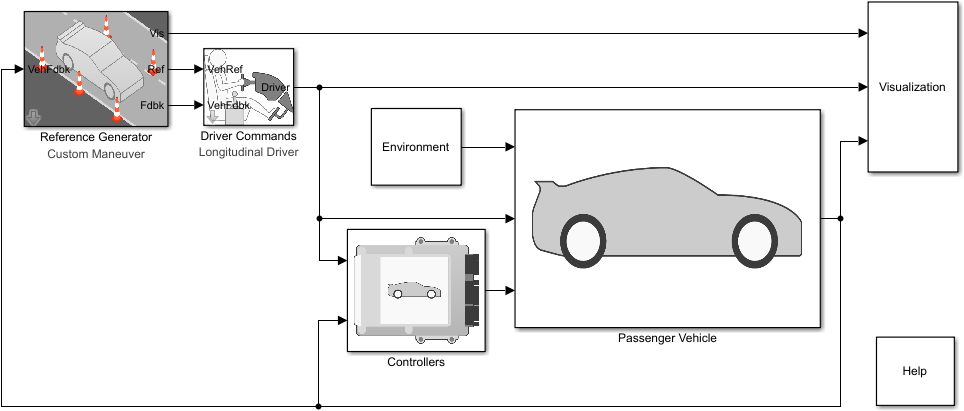
\includegraphics[width=0.9\textwidth]{Images/Simulator/sim-full}
	\end{center}


		\subsection{Passenger Vehicle}
		\label{ssec:vs-env-passveh}

		The core of the simulator resides inside the \emph{Passenger Vehicle} block.
		Besides the simple look of the cover image, this subsystem is a fine-grained model of a passenger car that reproduces not only the motion of a body in a 3D world,
		but every dynamic behavior of typical vehicle subsystems.

		The whole model is divided in two main sub-blocks. The \emph{Body} sub-block models the behavior of the unpowered chassis, in particular the suspension-road-tires
		interaction, extracting the resultant forces acting on the body given the drive torque. These forces are then processed by the \emph{Vehicle Body 3DOF} block to
		update the course taking into account additional phenomena including wind conditions, road incline and friction coefficients for each wheel (these two can be even
		extracted from real-time interaction with the 3D environment).

		The Body sub-system works on pure force and torque inputs, which are primarily provided by the second main piece: the \emph{Driveline}.
		This part translates typical controls available to a human driver into final wheel drive torques and brake commands by simulating the whole powertrain.
		It features both spark- and compression-ignition engines with mapped cycles, a fixed gear transmission and various differential flavors, all selected through variants.
		It also models the steering mechanism from driver to the wheels according to three different schemes, namely \emph{Parallel}, \emph{Rack-and-Pinion} and
		\emph{Ackerman}.

		The remaining sub-blocks are just signal pass-through boxes that route monolithic, high-level busses to their corresponding I/O ports. As such, these formal subsystems
		are of little functional significance and quite self explanatory.


		\subsection{Controllers}

		In the \emph{Controller} block are housed all the typical electronic control units found on modern cars. The most typical one is the \emph{Anti-lock Braking System},
		but there are also the differential control and others. 
		\begin{center}
			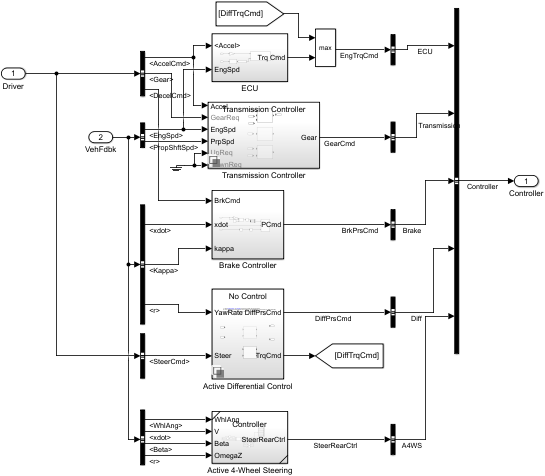
\includegraphics[width=0.9\textwidth]{Images/Simulator/ctrl-full}
		\end{center}

		Even though physically separated from the rest of the vehicle model, it is tightly coupled with that one, as it would be in the real world. As said before, any of these ECUs
		can be enabled through the corresponding variants.

		\subsection{Driver}
		\label{ssec:vs-env-drv}

		The \emph{Driver} block does exactly what it says, it drives the vehicle according to a provided reference path.
		The available variants include a \emph{Predictive Driver} that follows a path by acting on both the speed commands and the steering wheel,
		a \emph{Longitudinal Driver} for speed profiles only and an \emph{Open-Loop Driver} which basically passes on external, raw commands to the vehicle
		while maintaining consistency with the signal interface.
		
		This is somehow the most enigmatic of the blocks, mostly in lateral driving situations. Our understanding is that the Predictiove Driver was designed only for
		lateral displacement driving actions like in lane change maneuvers. However, the \emph{Constant Radius} reference application features an active curved-trajectory
		scenario where the Predictive Driver is employed through a mangling of the feedback signals from the vehicle, tricking the driver into a sort of constant lane change. As
		we'll better explain in~\vref{ssec:vs-int-cm}, the complex algorithm for predictive driving often reached an unstable situation, jeopardizing any good result in our work.


		\subsection{Reference Generator}

		Here is where the director leads the orchestra. Despite the humble name, the \emph{Reference Generator} does much more than simply provide the reference path
		to the driver. It actually offers the main settings panel for selecting the type of maneuver, the 3D scenario and the simulated vehicle model, the cruise speed and specific
		maneuver parameters. In the background, each callback to the scripts changes accordingly the remaining blocks of the simulator to meet the requests.
		\begin{center}
			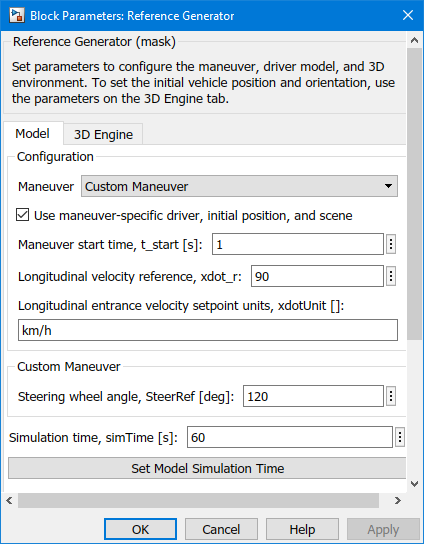
\includegraphics[height=0.3\textheight]{Images/Simulator/sim-refgen-cfg}
		\end{center}


		\subsection{Visualizer}

		The last component of the simulator is the \emph{Visualizer}, the most user-friendly of them all. Apart from collecting each and every useful signal from the whole system,
		the Visualizer offers a real-time dashboard showing the state of the car.
		\begin{figure}
			\centering
			\subfloat[][]{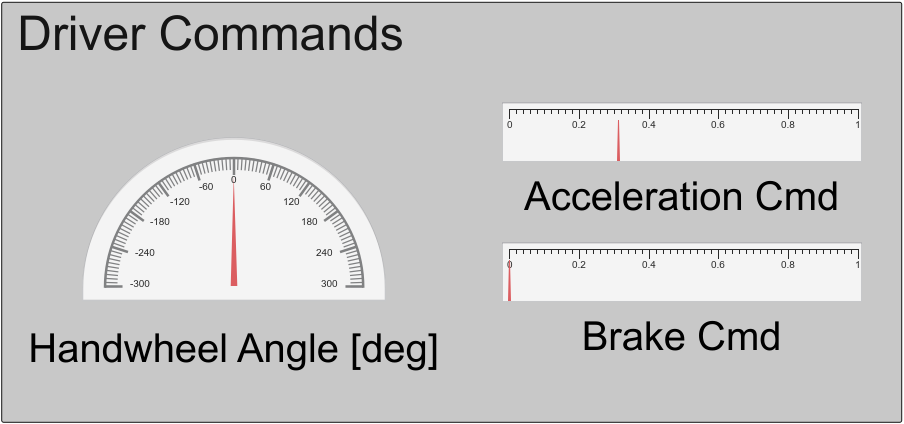
\includegraphics[height=0.12\textheight]{Images/Simulator/vis-dash-drv}}\quad
			\subfloat[][]{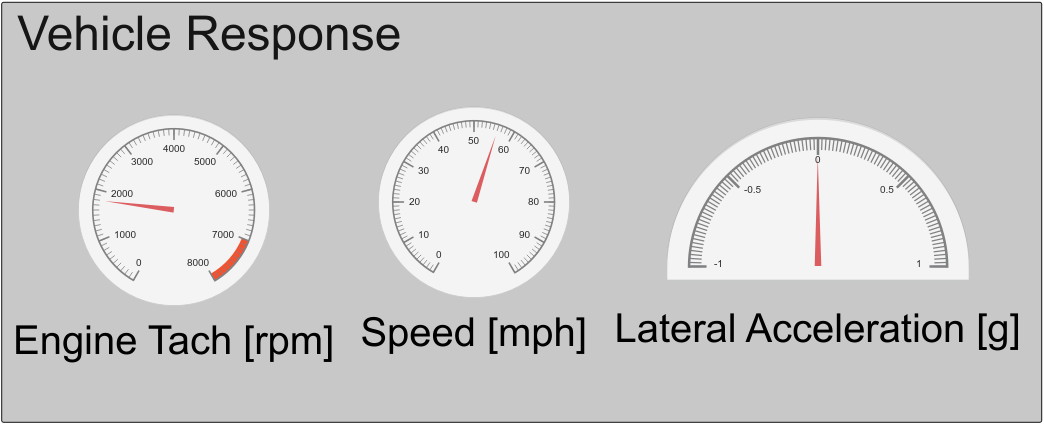
\includegraphics[height=0.12\textheight]{Images/Simulator/vis-dash-veh}}
		\caption{Detail of the real-time dashboard}
		\label{fig:vis-dash}
		\end{figure}
%		\begin{figure}
%			\centering
%			\subfloat[][]{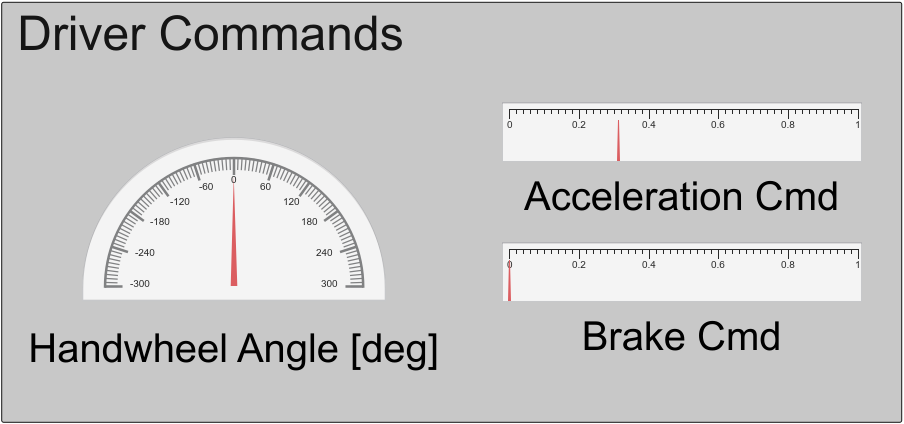
\includegraphics[width=0.45\textwidth]{Images/Simulator/vis-dash-drv}}\\
%			\subfloat[][]{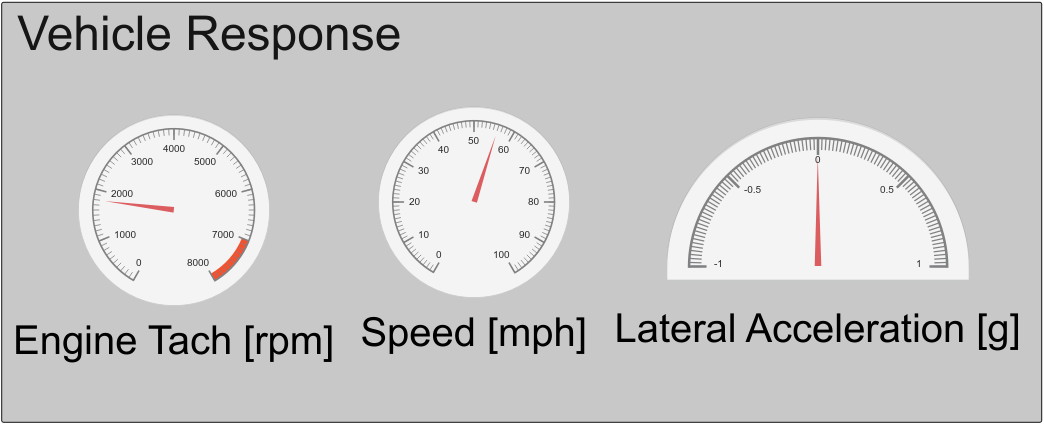
\includegraphics[width=0.45\textwidth]{Images/Simulator/vis-dash-veh}}
%		\caption{Detail of the real-time dashboard}
%		\label{fig:vis-dash}
%		\end{figure}

		It also implements all the machinery required to interface with the Unreal Engine 4 for realistic
		3D visualization of the whole action.


	\section{Integration}
	
	The framework described so far makes for a very flexible environment, yet it hardly satisfies our requirements out of the box.
	Yet, we wanted to preserve as much of the original functions as possible, with targeted inclusions rather than outright changes, sticking to the original structure and layout.
%	To blend seamlessly in such a sophisticated system, we performed some important changes in key components following the logical partitioning as much as possible.
	The first step to keep the reference application clean is to reference its project file from within ours. This technicality boils down to a \mwSL{} model with a single block
	referencing to the simulator top-level model, to establish the dependency. For all the other development purposes, \texttt{model/A4WS.slx} is a mere placeholder and the
	\lstinline{CRReferenceApplication} block should be opened as the top-level model each time through the dedicated button in the bottom-left corner.


		\subsection{Rear Steering}
		
		First and foremost, we needed a rear-steered car. Since an active rear-steering control is still uncommon, the original simulator had no variant for that and required some
		\mwSL{} plumbing. Nonetheless, the Passenger Vehicle~\ref{ssec:vs-env-passveh} subsystem follows a redundant but consistent structure and provides a signal bus
		for all four wheel angles, among others. This helped a lot, since we just had to arrange a dedicated \emph{Kinematic Steering} for the rear wheels inside the
		\emph{Driveline}, replace the grounded wheel signal with its output and finally route the input up to our control unit (see below), following all translation stages and bus
		aggregations.
		\begin{figure}
			\centering
			\subfloat[][Rear Steering signal routing]{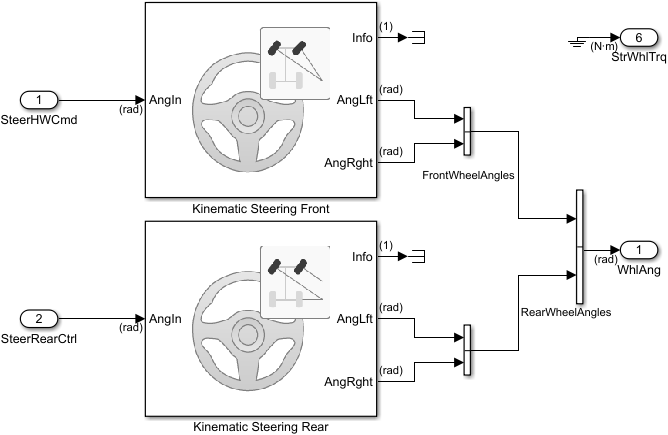
\includegraphics[width=0.45\textwidth]{Images/Simulator/veh-drvln-steer}}\quad
			\subfloat[][Body model adaptation]{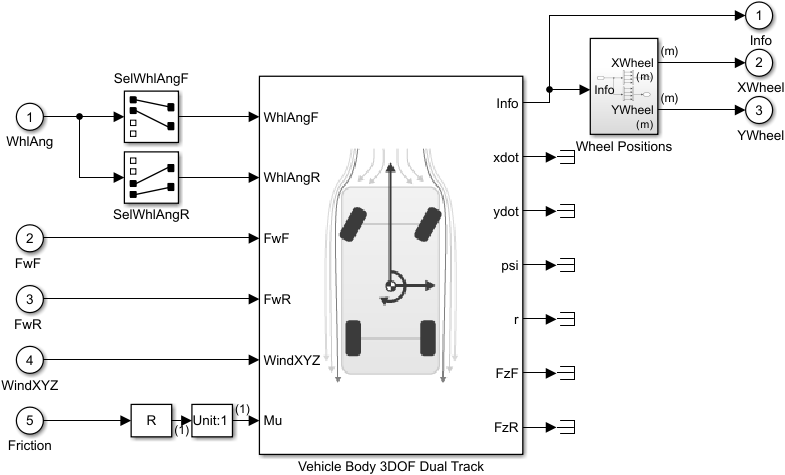
\includegraphics[width=0.45\textwidth]{Images/Simulator/veh-body-detail}}
		\caption{}
		\label{}
		\end{figure}

		The Kinematic Steering for the rear wheels is set to a ratio of 1:1 for direct wheel control, while saturating the maximum steering range according to the
		\lstinline{rngRearSteer} parameter in \texttt{model/SimRoutine.m} (the default range is $\pm\ang{5}$). A counterintuitive setting is the \emph{Front} option,
		which ensures the wheels get the angle signal of the same sign as the control output.


		\subsection{A4WS Control Unit}
		\label{ssec:vs-int-ctrl}

		Consistent with the overall layout, our \emph{\awwwws} control unit is located inside the Controllers block with all the other ECUs.
		Basically, it is a separate \mwSL{} sub-model inside \texttt{model/Controller.slx} enclosing our development into a separate container, for better abstraction.
		The block taps into the vehicle \emph{feedback bus} to retrieve the required system data, namely \emph{speed}, the \emph{side-slip angle} and \emph{yaw rate},
		while the \emph{rear-steer angle} output is included in the \emph{Controller} bus with the dedicated \lstinline{A4WS/CmdRearSteer} channel and reaches the kinematic
		steering element in the driveline subsystem (see above).

		Inside \texttt{model/Controller.slx} the actual control block --- a \emph{\mwML{} Function} --- communicates with the outside world through two translation blocks.
		These subsystems take care of proper unit conversion and reference frame translation, as the whole simulator is built around a down-pointing frame, while we felt
		more comfortable with the usual choice of the Z axis pointing against gravity. Luckily, the signals involved include only yaw angles and changing the sign does the job.
		\begin{center}
			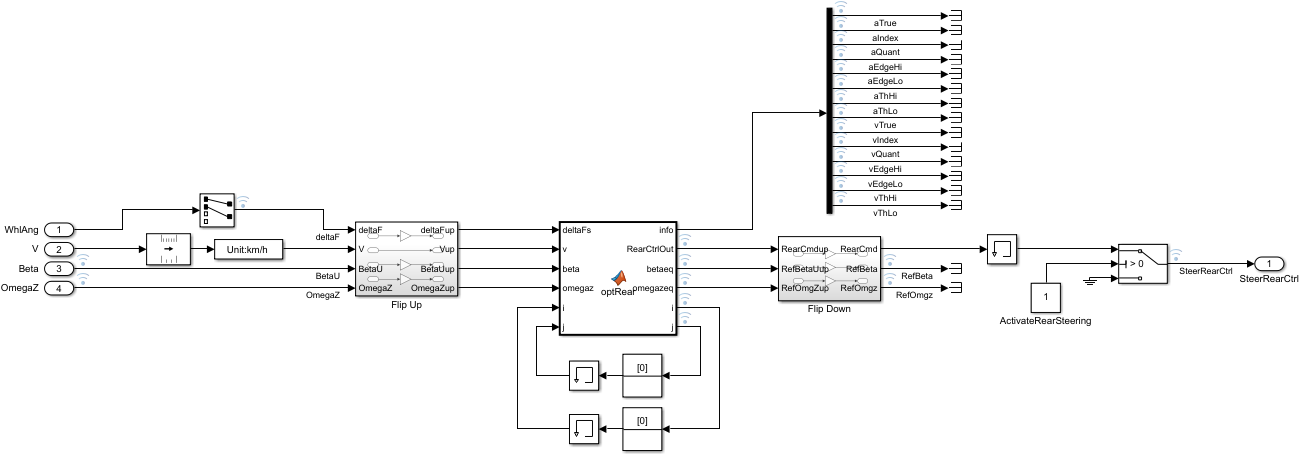
\includegraphics[width=0.9\textwidth]{Images/Simulator/a4ws-full}
		\end{center}

		The beefy part of the controller is inside the function block \lstinline{optRear} and, as the name suggests, it is where the state is fed back to the system scaled by a scale
		matrix, obtained through optimal control as described in \vref{sec:vs-ctrl}. Prior to this, two important action are performed.
		First, the right gain coefficients are picked from the look-up table \lstinline{Klut}, according to the mean-value of the current front wheel angles and the speed.
		To avoid harmful glitches, there is a hysteretic mechanism that switches to another gain matrix K only if the threshold has been crossed with enough margin.
		\lstinputlisting[firstline=7, lastline=41, firstnumber=7]{Images/Simulator/a4ws-code.m}
		The inner workings of this selection process are made available at the \lstinline{info} port and features two sets of seven values for the true value, the quantized one,
		the would-be index and the upper and lower values for both the division boundaries and the thresholds.
		\lstinputlisting[firstline=43, lastline=43, firstnumber=43]{Images/Simulator/a4ws-code.m}
		
		The settings for these threshold, expressed in percentage over one division of the full range, can be found at the very beginning of \texttt{model/SimRoutine.m}:
		\lstinputlisting[firstline=9, lastline=15, firstnumber=9]{../../../model/SimRoutine.m}
		
		The second step is to extract the instantaneous equilibrium point by inverting on-the-fly the matrix $A$, to adapt the reference signals to external conditions as well:
		\lstinputlisting[firstline=46, lastline=86, firstnumber=46]{Images/Simulator/a4ws-code.m}
		
		Once the controller have all the ingredients ready, the usual operation $u = -Kx$ is performed and returned at the output:
		\lstinputlisting[firstline=90, firstnumber=90]{Images/Simulator/a4ws-code.m}


		\subsection{Custom Maneuver}
		\label{ssec:vs-int-cm}

		Unfortunately, the provided scenarios where difficult to use out-of-the-box, so instead of radically changing them we decided to add our custom maneuver.
		It might seem a straightforward approach, yet there are a fair amount of cross-scripts to take care of to make the new scenario fit in the simulator.
		By examining the \emph{mask layout} of the Reference Generator block, we were able to track all the script involved and mirror the required actions on our case.
		
		Most notably, we choose to set the Driver to a Longitudinal one and provide direct signals for the steering wheel. The initial hype for the Predictive Driver faded as
		we experienced more and more instability during early simulations. The algorithm implemented in such advanced driver model was hard to interpret and fix, so we traded
		off some realism for quicker results. Moreover, the block is intended for lateral references along a straight path, like lane-change maneuvers on a highway.
		As mentioned in \vref{ssec:vs-env-drv}, the \emph{Constant Radius} maneuver uses a Predictive Driver to achieve a circular path, by overriding the feedback signals
		from the vehicle and tricking the driver into perceiving the car on a straight road and feeding back the turn reference as a constant displacement from the centerline.

		Once the Predictive Driver got discarded, we moved on to implement our reference maneuvers. Again, we took advantage of \mwSL{} model variants to create a set of
		simple patterns, yet perfectly repeatable and simple to interpret. They sum up to:
		\begin{description}

			\item[Constant] The steering wheel is kept constant for the whole time;

			\item[2-Step] The steering wheel briefly steps to the given angle a quickly settles to its double for the rest of the time;

			\item[Lane-Change] The vehicle is steered first to the given direction, then straightened up and finally steered back to the starting lane after ten seconds;

			\item[Evasive] Similar to the lane-change maneuver, but reverts to the original lane much quicker, similarly to an obstacle avoidance action.

		\end{description}
		
		Each maneuver is initiated at time \SI{20}{\second} and both the \emph{speed} and \emph{steering wheel angle} are set in the Reference Generator settings dialog.
		The time delay is to let the speed build up before system excitation. For the more articulated maneuvers, the steering profile is obtained by a chain of step generators
		compensating each other at different time steps. It's a crude yet effective way to lay a pattern and despite the unrealistic step variation of the steering, this ensures that
		good results could only improve with smoother excitation.
		\begin{center}
			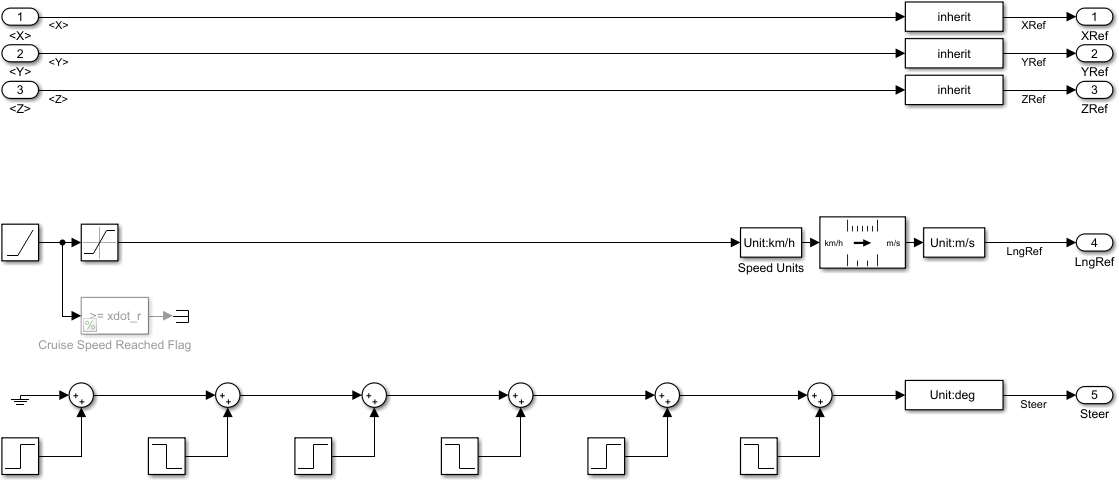
\includegraphics[width=0.9\textwidth]{Images/Simulator/cm-s-full}
		\end{center}


		\subsection{Environment}

		In a very similar way to the steering patterns in the previous section, we implemented also a set of adverse environmental conditions.
		Even if logically implemented in distinct sub-blocks, we list them altogether:
		\begin{description}

			\item[No Wind] The aerodynamic force is completely suppressed;

			\item[Lateral] The vehicle is subject to a constant wind, blowing in the negative lateral direction;

			\item[Burst] Same as Lateral wind, except the vehicle experiences a brief burst of wind;

			\item[Ideal Road] The road presents a unit scaling factor for the tire friction force;

			\item[Ice Patch] The car travels through an icy patch and then recovers traction;

			\item[Snowy Range] The road switches from tarmac to snow for the rest of the time.

		\end{description}
		
		Again, these disturbances kick in few seconds after the maneuver is initiated, to let the vehicle build up some spin and make the effect more dramatic.
		As usual, model variants lets the two phenomena combine together at will.
		\begin{figure}
			\centering
			\subfloat[][\lstinline{Environment} block]{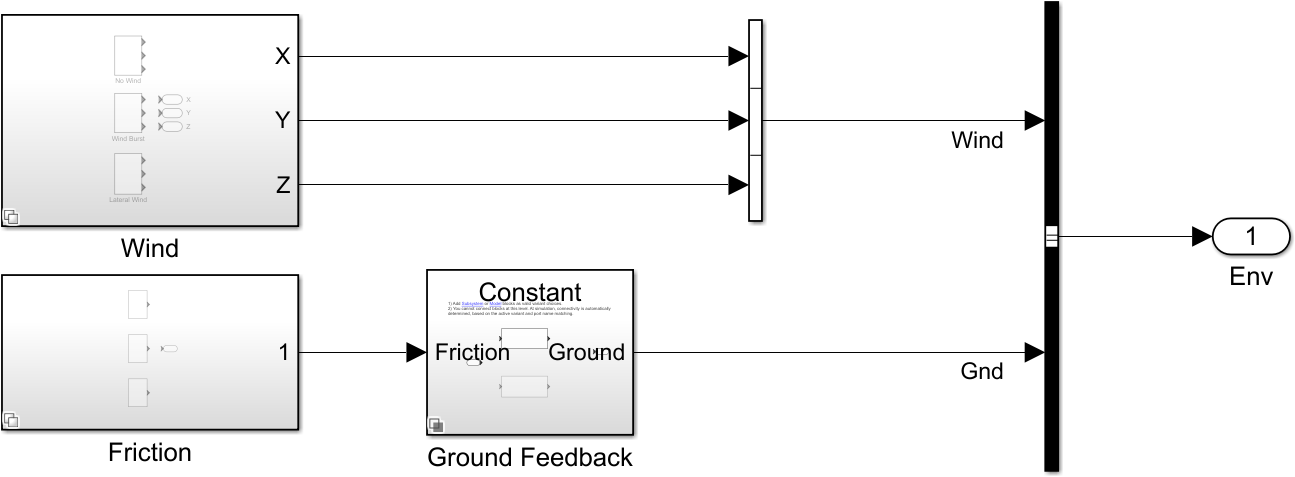
\includegraphics[width=0.55\textwidth]{Images/Simulator/env-full}}\quad
			\subfloat[][\lstinline{Wind Burst} sub-block]{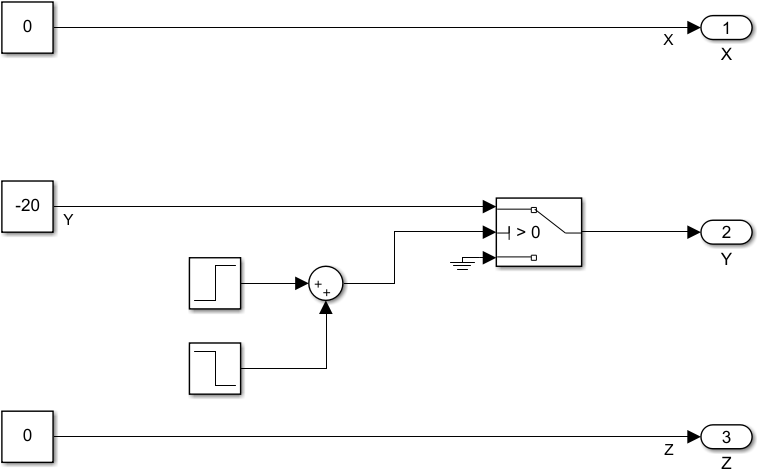
\includegraphics[width=0.35\textwidth]{Images/Simulator/env-wind-burst}}
		\caption{}
		\label{}
		\end{figure}


	\section{Control}
	\label{sec:vs-ctrl}

	The last, crucial component that completes our project is a set of scripts that perform calculus and drive the simulator to obtain the resulting data.
	The entry point for the whole simulation is \texttt{model/SimScript.m}, which first extracts vehicle parameters from the model workspace and sets some constants for the size and
	the resolution of the control look-up tables (as seen in \ref{ssec:vs-int-ctrl}):
	\lstinputlisting[firstline=7, lastline=19, firstnumber=7]{../../../model/SimRoutine.m}
	Then, it hands all the parameters to the optimization engine:
	\lstinputlisting[firstline=21, lastline=22, firstnumber=21]{../../../model/SimRoutine.m}
	Finally, the simulation sequence is launched:
	\lstinputlisting[firstline=25, lastline=29, firstnumber=25]{../../../model/SimRoutine.m}
	The rest of the code formats the output data and plots the results. Its expansion \texttt{model/SimRoutine2.m} automates the simulation for different environmental conditions.
	
	The optimization engine takes an intermediate step inside \texttt{model/LUTScript.m}, which populates the look-up table used by the controller with the gain coefficients.
	These are obtained from subsequent invocations of \texttt{model/LinPlant.m}:
	\lstinputlisting[firstline=1, firstnumber=1]{../../../model/LUTScript.m}
	Here the vehicle body dynamics are linearized around the provided point and control law
	parameters are calculated through \emph{Optimal Control} methods, namely the \lstinline{lqr} \mwML{} function.
	% !TEX encoding = UTF-8 Unicode
% !TEX TS-program = pdflatex
% !TEX spellcheck = en-US
% !TEX root = ../Report.tex

\chapter{Optimal Control Design}
Inside this chapter, we are going to show the control system we designed for our application. This phase has been the most complex one for different reasons. Generally speaking, the design of a specific control law for each physical system depends by many factors, having different levels of influence. For this reason, we tried to design the best possible control law by considering more the most important elements and neglecting and/or minimizing the ones with a low impact. As a consequence, this step required us lots of time to be fully accomplished.\\
At first we brought our devised system into Matlab, initializing all these variables able to influence its behaviour, so that the control system could act over a vehicle model that was similar to the one used by the simulator. Then, we built the handles to connect them with the simulator in order to achieve a simulation environment inside which we could test our control system in comparison with an open loop simulation. Moreover, we merged the simulator and the control law together in Simulink and we started optimizing the system. Finally, after some considerations, we have implemented also the disturbance compensation since, in our case, we knew its value a priori. In this way, we could reach an optimal control system acting on the \textit{state} variables by considering also the influence given by the human driver, $\delta_{wf}$.\\
\begin{figure}
		\centering
		\lstinputlisting[caption={[SimDataImport]}, firstline=28, lastline=32, firstnumber=28]{../../../model/LinPlant.m}
		\caption{Import vehicle data from the simulator}
		\label{stability}
	\end{figure}
\section{Control Law design}
This step was the most critical one because of its close correlation with the project purpose itself. Our starting object was to develop a control law able to act over the steering angle of the rear wheels, $\delta_{wr}$. We chose to use the Optimal Control Law because that's what we have been presented during the course. In the following paragraphs there will be a brief description of our procedure. In particular, we didn't apply a simple opìtimal control to reduce the erros
\section{Cost Function $J$ Analysis}
Starting from the theory, we studied the real meaning of "Cost Function" and its elements. The function's goal is to design a control system, $u$, ables to minimize the function $J$ itself. In a nutshell, if a certain condition is strongly desired, we have to associate to it a low cost, and viceversa. \\
There follow the linear quadratic form of the cost function $J$ for a general LTI system:
\begin{equation}
J = x^{T}(t_{f}) S_{f} x(t_{f}) + \int_{t_{0}}^{t_{f}} e^{T} Q e + u^{T} R u \ dt
\end{equation}
where:
\begin{itemize}
	\item $e$ represents a linear combination of \textit{states} x;
	\item $u$ represents the control law;
	\item $ [t_{0},t_{f}] $ represents the time spain in which we evaluated our cost function J;
	\item $ S_{f} = S_{f}^{T} \geq0 $ represents the cost associated to the state once it is evaluated in $t=t_{f}$, so "how much far i am from the origin";
	\item $ Q=Q^{T}\geq 0 $ and $ R=R^{T}\geq 0 $ represent, respectively, the costs for having $e\neq0$ and $u\neq0$, during the time span.
\end{itemize}
\section{Q and R Matrices}
We could reach our final goal, in terms of meaningful imposed rear steering angle, through the "tuning" process of matrices $Q$ and $R$. For what concern the matrix $S$, we set it equal to zero because we didn't need to evaluate the error on the final condition, only during the evolution of the System, so we focused on Q and R matrices. In particular, we started with the rule of thumb of setting the values of these matrices a the inverse of the maximum error we could accept on the states and the inverse of the maximum control we could apply
\begin{equation} \label{Q MAtrix}
	\ Q =
	\begin{bmatrix}
	\ Q_{11} & 0\\
	\ 0 & Q_{22}
	\end{bmatrix} = \frac{1}{2}
	\begin{bmatrix}
	\ inv(max(\beta_{u}-\beta_{u_{ref}})) & 0\\
	\ 0 & inv(max(\omega_{z}-\omega_{f_{ref}}))
	\end{bmatrix}
\end{equation}
\begin{equation} \label{R MAtrix}
	\ R =
	\begin{bmatrix}
	\ R_{11}
	\end{bmatrix} =
	\begin{bmatrix}
	\ inv(max(\delta_{r}))
	\end{bmatrix}
\end{equation}
Q is a diagonal matrix, where $ Q_{11} $ represent the cost of being distant from the equilibrium state of $ \omega_{z} $ and $ Q_{22} $ represents the cost of being distant from the ideal $ \beta_{u} $. $ R_{11} $ instead is relative to the control.
The tuning first steered $ R_{11} $ in order to keep it inside the physical bounds that we decided to set (still tunable, but set 5° in the definitive form), then we modified $ Q_{11} $ and $ Q_{22} $ one in relation with the other, in order to get the best possible compromise.
\section{K multiplier}
Following the theory of optimal control we should extract one single K matrix around the linearization point. This made our working condition very limited, because, by choosing a linearization point, we would have to choose one single steering angle and angular velocity. This condition was restricting the validity range of our system around a certain kind of curve, that initially has been specified as a straight trajectory ($\omega_{z}=0$).
This reason led us towards the consideration of extracting not one matrix for K, but a whole range of values, based on two inputs from the driver:
\begin{itemize}
	\item front steering angle: $\delta_{wf}$;
	\item current vehicle speed: $V_0$.
\end{itemize}
This extraction is not done in real time, due to the relatively high computational load of performing an LQR algorithm. It, instead, is done only once at the startup of the system (now that we are in prototypation phase, later on it will only be performed once and for all). After this initial computations made at some discrete linearization points, the results will be stored in lookup tables and, at run-time, the only workload for the microcontroller will be to take as input the actual state of the machine (specifically the two input parameters written in the bullet list here above) and perform matrix multiplication as usual.\\
Obviously, given the discrete nature of the lookup table, it will not be possible to have a perfect match for the actual disturbances of the vehicle that span across a continuous space, so we will have to approximate to the nearest point of linearization. It will be anyway a better approximated solution with respect to a system with a single linearization point and a single K.\\
Another reason why we have devoted one script for the extraction of K matrices and another one for the computation of realtime control is that you can't generate C code using matlab coder or even a simulink block with Matlab code containing the lqr algorhytm present in the control system toolbox. We needed to keep it separate.\\
Anyway due to the continuous variation of the equilibrium states, we dont'have big problems on the steep variation of controls.
\begin{figure}[!h]
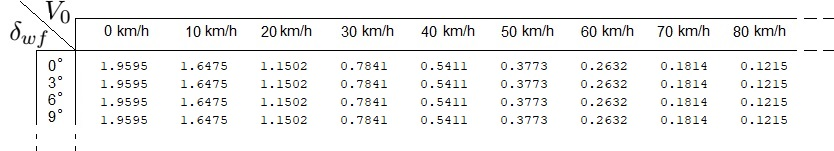
\includegraphics[width=\linewidth]{../Images/KLut.jpg}\caption{Excerpt of K Lookup Table}
\end{figure}
\section{H multiplier} \label{H section}
As we introduced at the beginning of current chapter, we have implemented also the disturbance compensation, due to $\delta_{wf}$, inside our control law. In particular, since we would like to reach a stable vehicle characterized by a constant $\omega_{z}$ (so that it is as similar as possible to $\omega_{z_{ref}}$), we focused our attention mainly on this \textit{state}. Therefore, this choice led us to compensate the disturbance effect mostly for $\omega_{z}$ \textit{state}. As well, even after this choice, we noticed that, also the $\beta_{u}$, has been correctly compensated.

Up to now, by means of the LQR optimal control system application, once the real working conditions differ from the equilibrium points we found, we can correct the vehicle behaviour. However, such a system always feels the presence of the external disturbance, $\delta_{wf}$. In order to make "disturbance-immune" (from $\delta_{wf}$ point of view, only) our controller, we computed the needed parameter to be added to our final control law. That parameter, \ref{HEquat}, has the purpose of considering the disturbance effect and compensating for it.
The following equations will better clarify this concept.

In order to correctly compute the H equation, we started from the following general equation:
\begin{equation} \label{StartEq}
	\dot{\tilde{x}} = A \tilde{x} + B_{1}\tilde{\delta_{wr}} + B_{2}\tilde{\delta_{wf}} = 0
\end{equation}
Then, we imposed the next equation as our "new" control law taking into account also the presence of disturbance:
\begin{equation} \label{new u}
	u = - K \tilde{x} + H \tilde{d}
\end{equation}
By including the equation \ref{new u} inside the \ref{StartEq} one, we obtained:
\begin{equation}
	\dot{\tilde{x}} = A \tilde{x} + B_{1}(- K \tilde{x} + H \tilde{d}) + B_{2}\tilde{\delta_{wf}} = 0
\end{equation}
Focusing our attention to H parameter, we reached the following final equation:
\begin{equation}
 (B_{1} H + B_{2})\tilde{d} = 0
\end{equation}
As we previously said, if we consider the disturbance compensation mainly for the $\omega_{z}$ \textit{state}, we finally obtain:
\begin{equation}
\label{HEquat}
H = -\frac{b_{{2}_{21}}}{b_{{1}_{21}}}
\end{equation}
\section{Saturation of control and states}
As we have already written before, we saturate the control signal to a physically feasible range of steering, but this is not enough. As a matter of facts, if the achieved results of the LQR algorithm computing $\omega_{z_{ref}}$ or $\beta_{u_{ref}}$ are out of any physically possible range, our control will always be saturated, thus not exercising the control that we should expect from it. For this reason we apply a saturation of the \textit{states}, depending on the vehicle velocity, like the one implemented in the ESP example.
\section{Resulting Control}
 Merging together all the previous concepts, we can actually show our final control law:
\begin{equation} \label{Resulting Control}
	\ \delta_{r} = -
	\begin{bmatrix}
	\ K_{1} & K_{2}
	\end{bmatrix}
	\begin{bmatrix}
	\ \beta_{u}-\beta_{u_{ref}} \\
	\ \omega_{z}-\omega_{z_{ref}}
	\end{bmatrix} +
	H \delta_{wf}
\end{equation}
Where:
\begin{itemize}
	\item K matrix is obtained from the lookup table generated at startup;
	\item $\beta_{u}$ and $\omega_{z}$ are the current \textit{state} values;
	\item $\omega_{z_{ref}}$ is the result of a real time computation of equilibrium states;
	\item $\beta_{u_{ref}}$, instead, is set equal to 0 because we would like to have the front of the car as aligned as possible with the direction of the velocity vector;
	\item H is the scalar multiplication factor described inside subsection \ref{H section};
	\item $\delta_{wf}$ is the system \textit{disturbance} variable "fixed", moment by moment, by human driver.
\end{itemize}

	% !TEX encoding = UTF-8 Unicode
% !TEX TS-program = pdflatex
% !TEX spellcheck = en-US
% !TEX root = ../Report.tex

\chapter{Final Results}
Inside this chapter,we are going to show the results of our work, analizing the states evolution making a comparison between the Open and Cloosed loop condition, focusing on the different trajectories performed by the vehicle. In order to analyze the behaviour of our vehicle we set five different scenery that resumes most of the real driving condition. In particular we have analyzed the behaviour of the vehicle during a constant radios turn and a double turn that can be used as well to simulate a possible overtaking or an obstacles avoidance. Moreover, using a dedicated simroutine, we also analyzed the worst driving conditions relative to these scanery, taking into account possible drive disturbance as wind or bad road conditions. \\ 
Our controller provides a very precise response to the system variations, the value of the control action is generated taking into account the real time value of $\beta_{eq}$ and $\omega_{eq}$ as reference. The steady state condition are reached with a time in the order of few seconds. For our simulation we set a reference longitudinal speed of 90 km/h and a driver command steering angle of 120°. These value can be changed as wish in order to analize all the driving condition comprised in our speed and steering angle ranges; the overall simulation time is 60s. Regarging to the disturbance, we choiced to simulate the two main maneuvers (single and double turn) with the contribute of bad road condition as snow and ice, changing the relative fiction coefficient in the Simulik blocks, moreover we also make a simulation to consider environment contribute, in this case we fixed a lateral wind disturbance since as we know, it can modify the amount of aerodynamic forces of the car leading to unstable behaviour as well. All the disturbance hit the vehicle during the maneuver's initial turning phase.\\
\\
Analyzing these graphs is possible to see how the system try to reach the reference path and how the controller action improve the overall performance, it’s possible to appreciate a better behaviour in terms of stability, indeed the vehicle trajectory is more coherent with the ideal path. The car makes the manuever in a more safe and comfortable way, even in presence of environment  disturbances, avoiding over-under steering behaviour. The overall system maintain a proper robustness thanks to the optimal control algorithm. Using the vehicle dynamics toolbox is possible to get also the 3D rappresentation of the vehicle behaviour, altought these simulation require a lot of computational time. To conclude we can say that we achieved our desired value in terms of resonable angular speed and side slip angle, moreover a more detailed tuning phase of the Q and R matrix inside the cost function implementation can allow to further improve the overall performances.    

\begin{figure}[!h]
\section{Single turn}    
		\centering
	        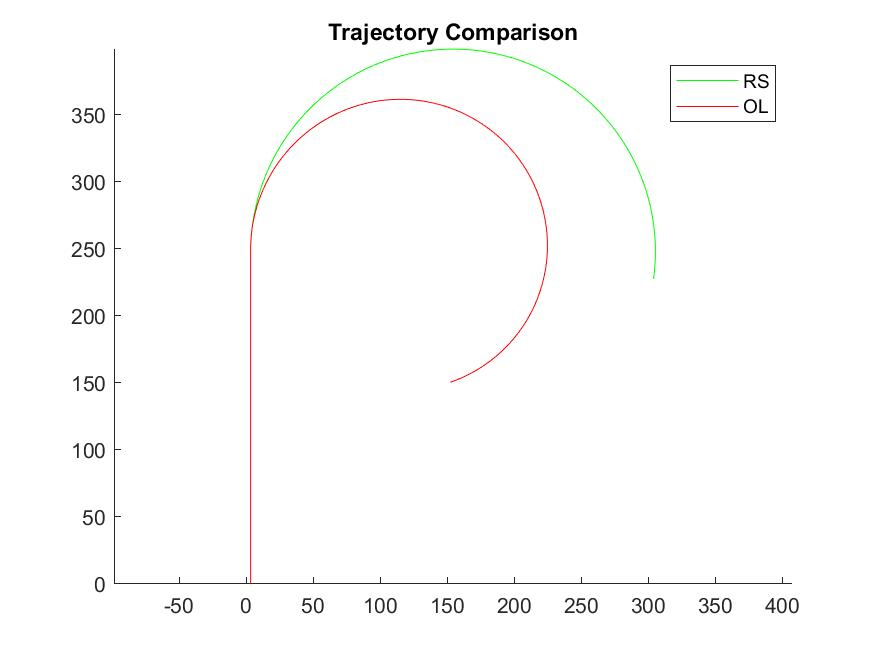
\includegraphics[scale=0.3]{./Images/ConstRadius/t} 
                \caption{(a)  RS vs OL comparison }
          
	\end{figure}

\begin{figure}[!h]
		\centering
	        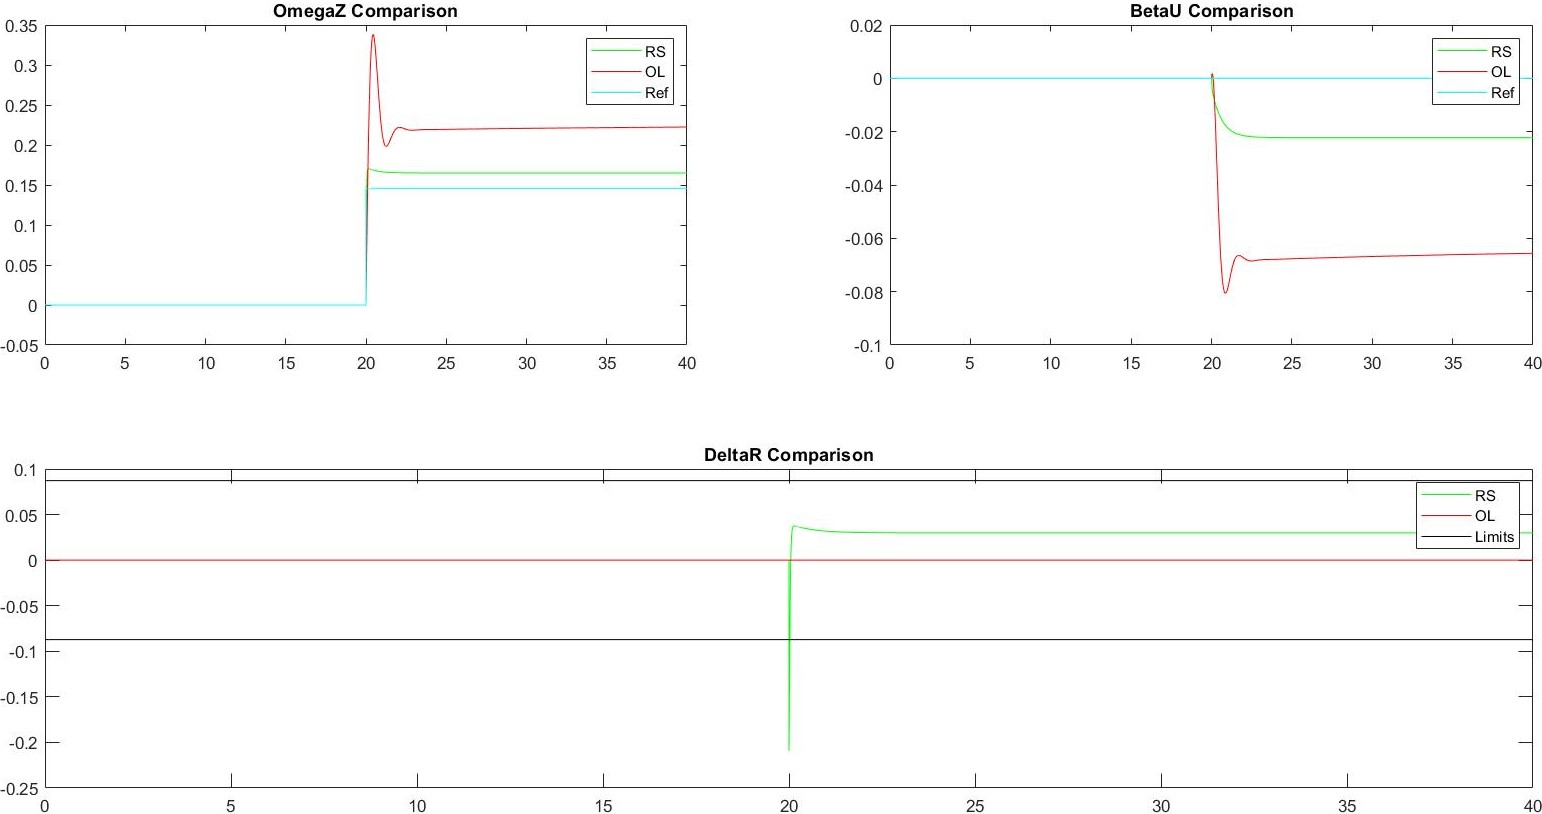
\includegraphics[scale=0.45]{./Images/ConstRadius/s} 
                \caption{(b)  Comparison of $\beta_{u}$, $\omega_{z}$ and $\delta_{r}$}
                \caption{Fig.1 Vehicle behaviour in constant radius scenario}
               
	\end{figure}

\begin{figure}[!h]
		\centering
	        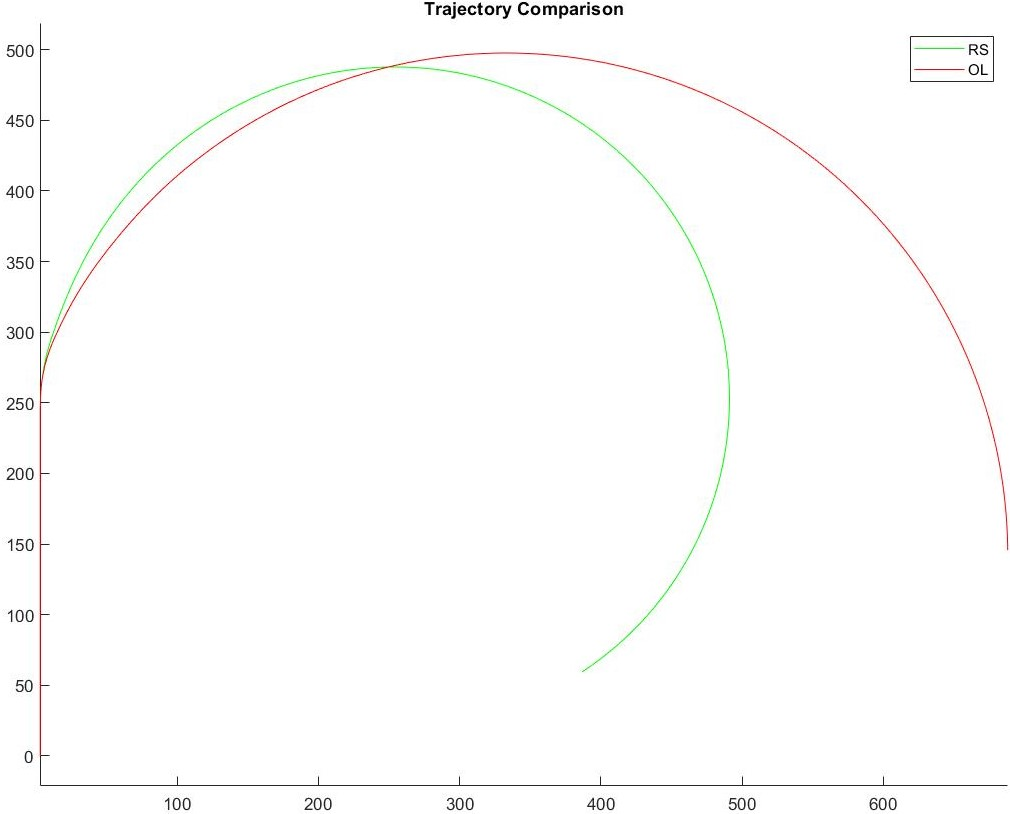
\includegraphics[scale=0.4]{./Images/ConstRSnow/t} 
                \caption{(a)  RS vs OL comparison}
          
	\end{figure}

\begin{figure}[!h]
		\centering
	        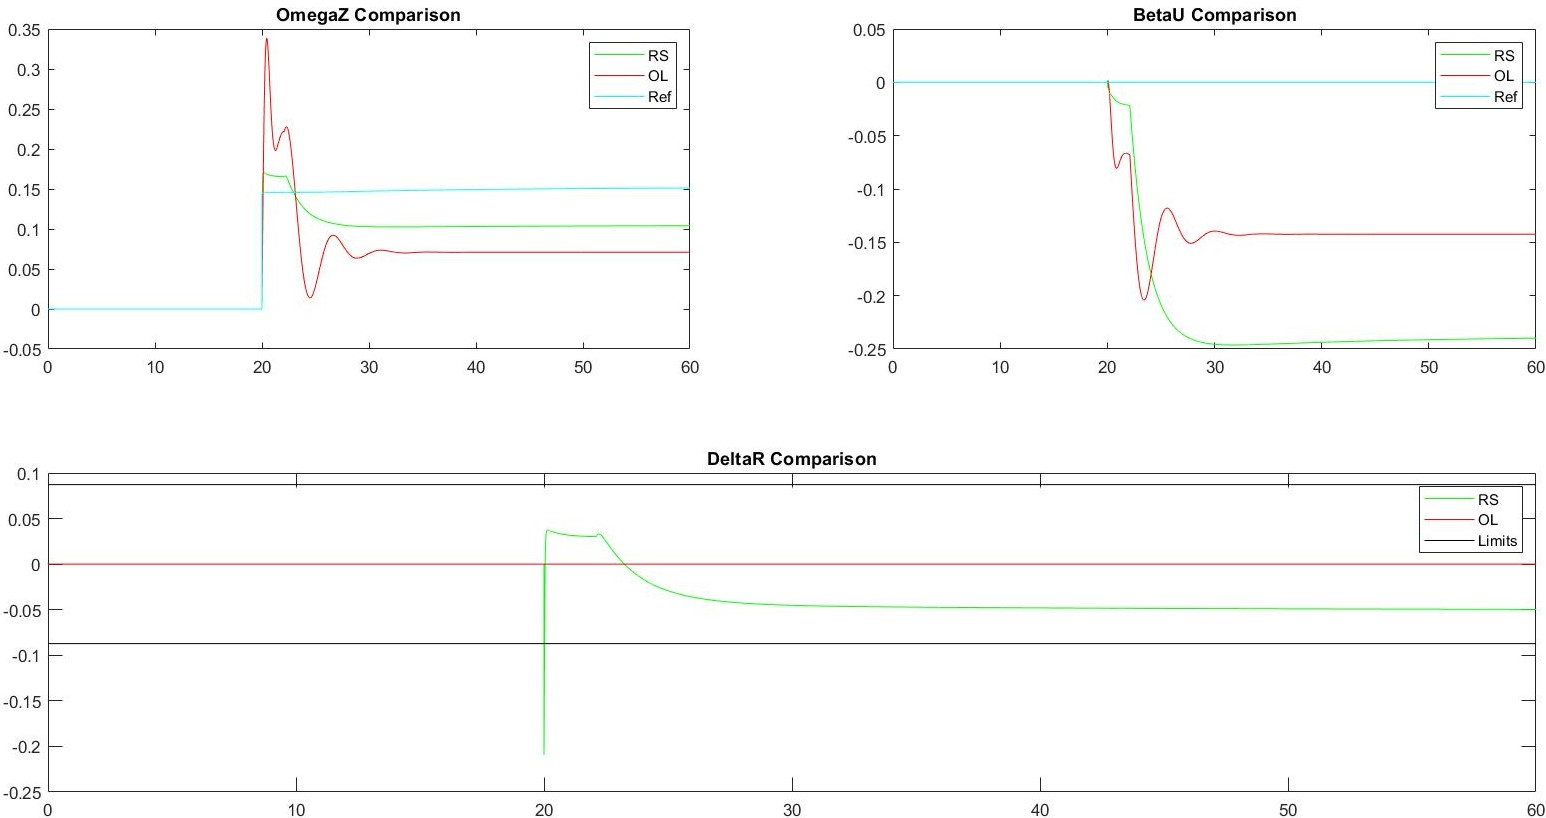
\includegraphics[scale=0.6]{./Images/ConstRSnow/s} 
                \caption{(b) Comparison of  $\beta_{u}$, $\omega_{z}$ and $\delta_{r}$}
                \caption{Fig.2 Constant Radius scenario with snow road}
               
	\end{figure}

\begin{figure}[!h]
		\centering
	        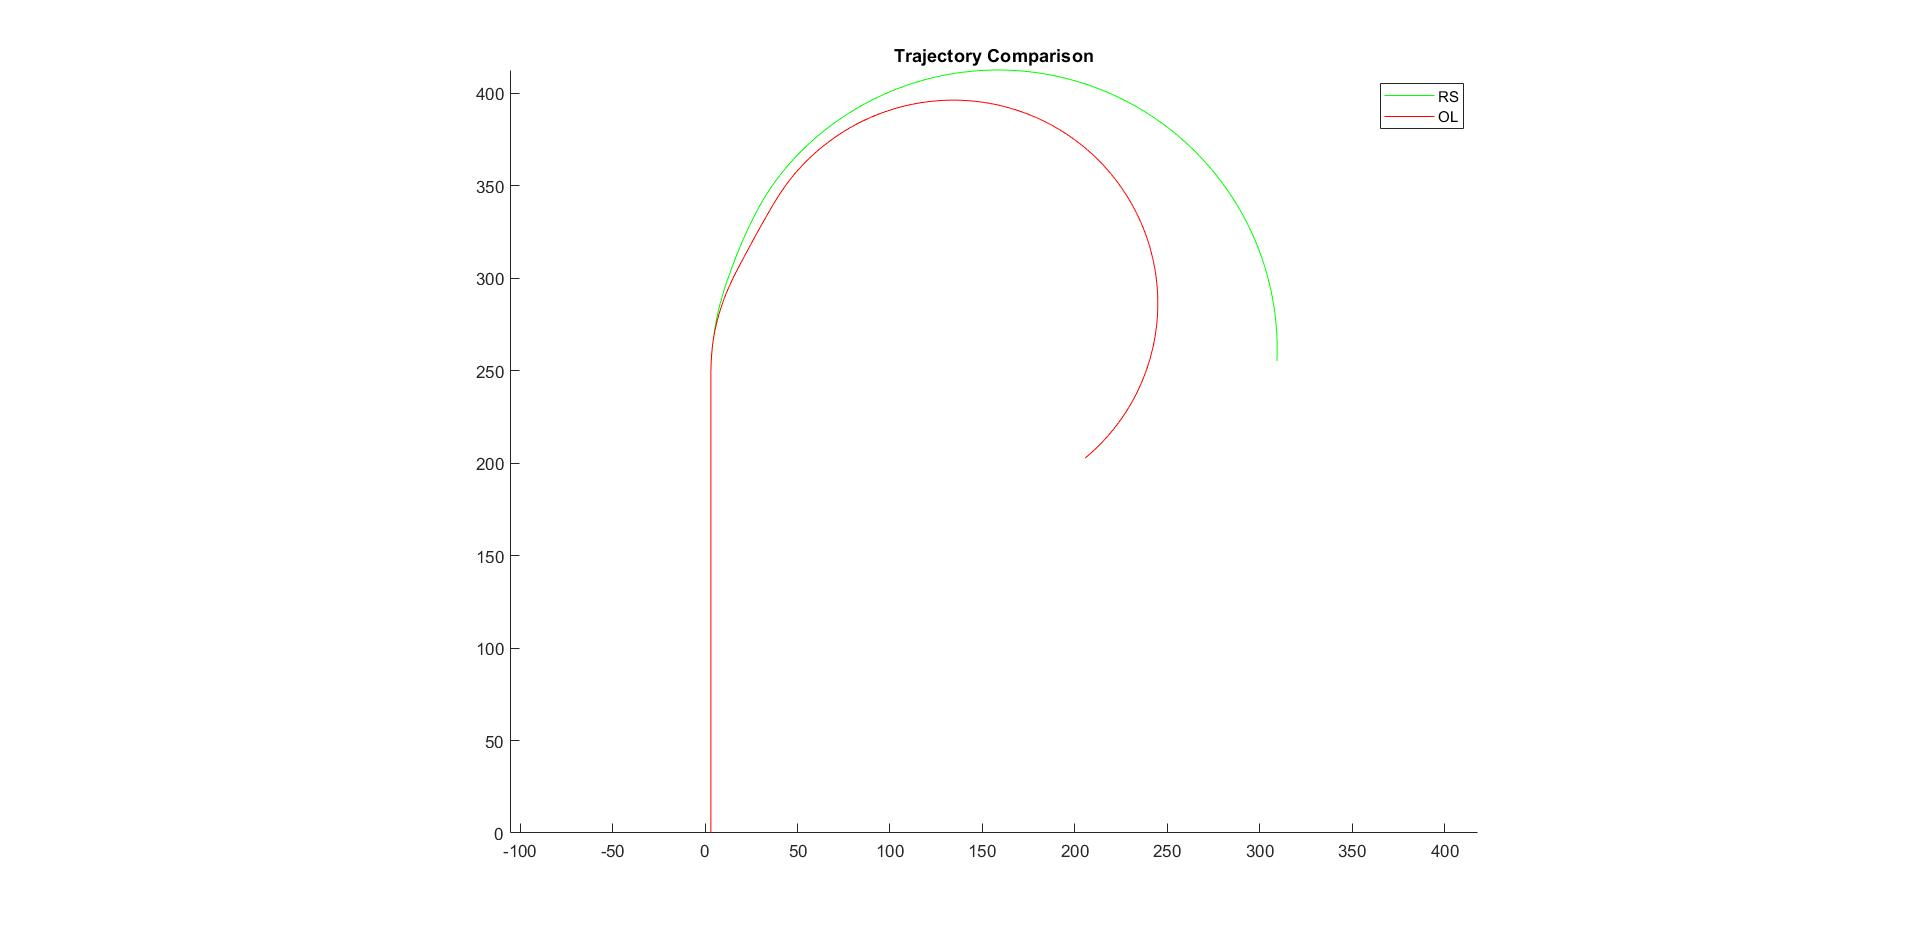
\includegraphics[scale=0.25]{./Images/ConstRwind/t} 
                \caption{(a)  RS vs OL comparison}
          
	\end{figure}

\begin{figure}[!h]
		\centering
	        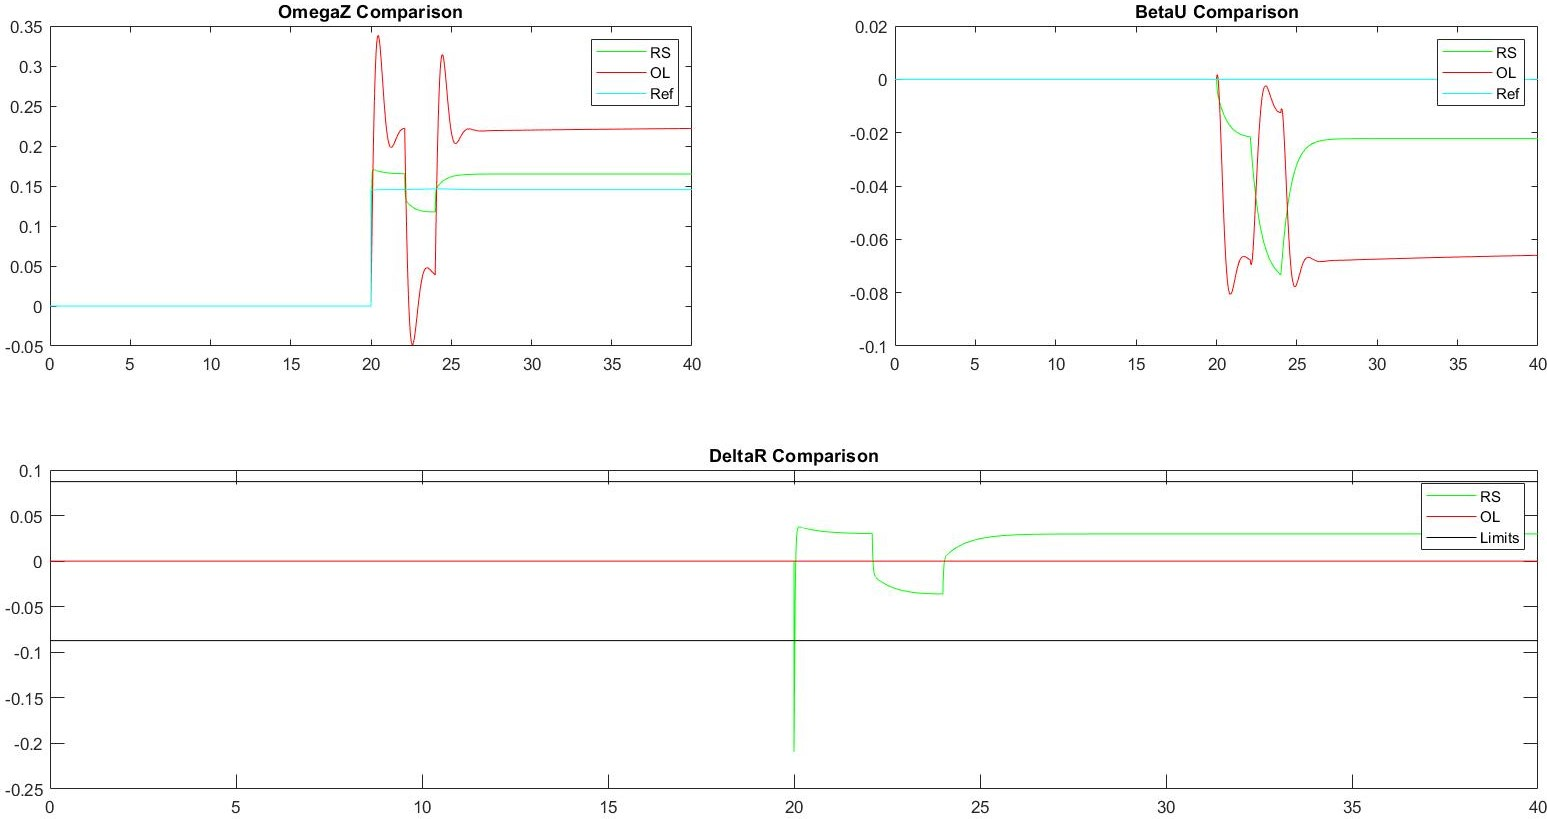
\includegraphics[scale=0.6]{./Images/ConstRwind/s} 
                \caption{(b) Comparison of  $\beta_{u}$, $\omega_{z}$ and $\delta_{r}$}
                \caption {Fig.3 Constant Radius scenario with lateral wind of 20 m/s}
	\end{figure}

\begin{figure}[!h]
\section{Double turn}
		\centering
	        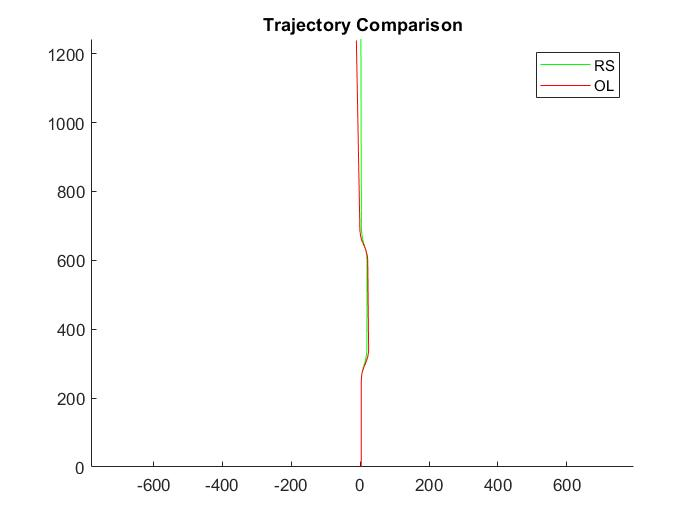
\includegraphics[scale=0.35]{./Images/LaneChange/t} 
                \caption{(a)  RS vs OL comparison}
             
	\end{figure}

\begin{figure}[!h]
		\centering
	        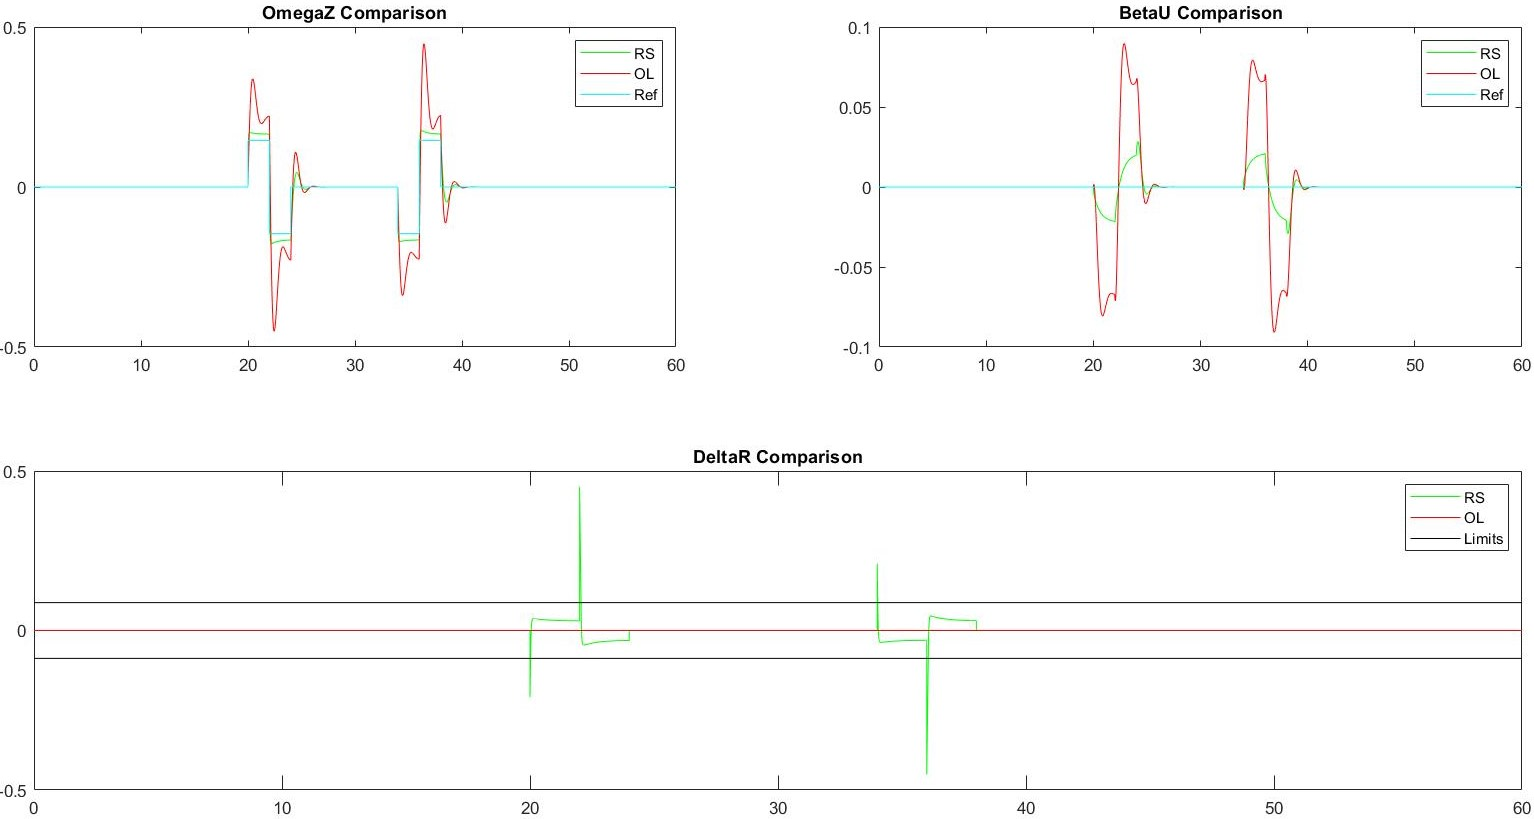
\includegraphics[scale=0.55]{./Images/LaneChange/s} 
                \caption{(b) Comparison of $\beta_{u}$, $\omega_{z}$ and $\delta_{r}$}
                \caption {Fig.4 Double turn witohut disturbance}
             
	\end{figure}

\begin{figure}[!h]
		\centering
	        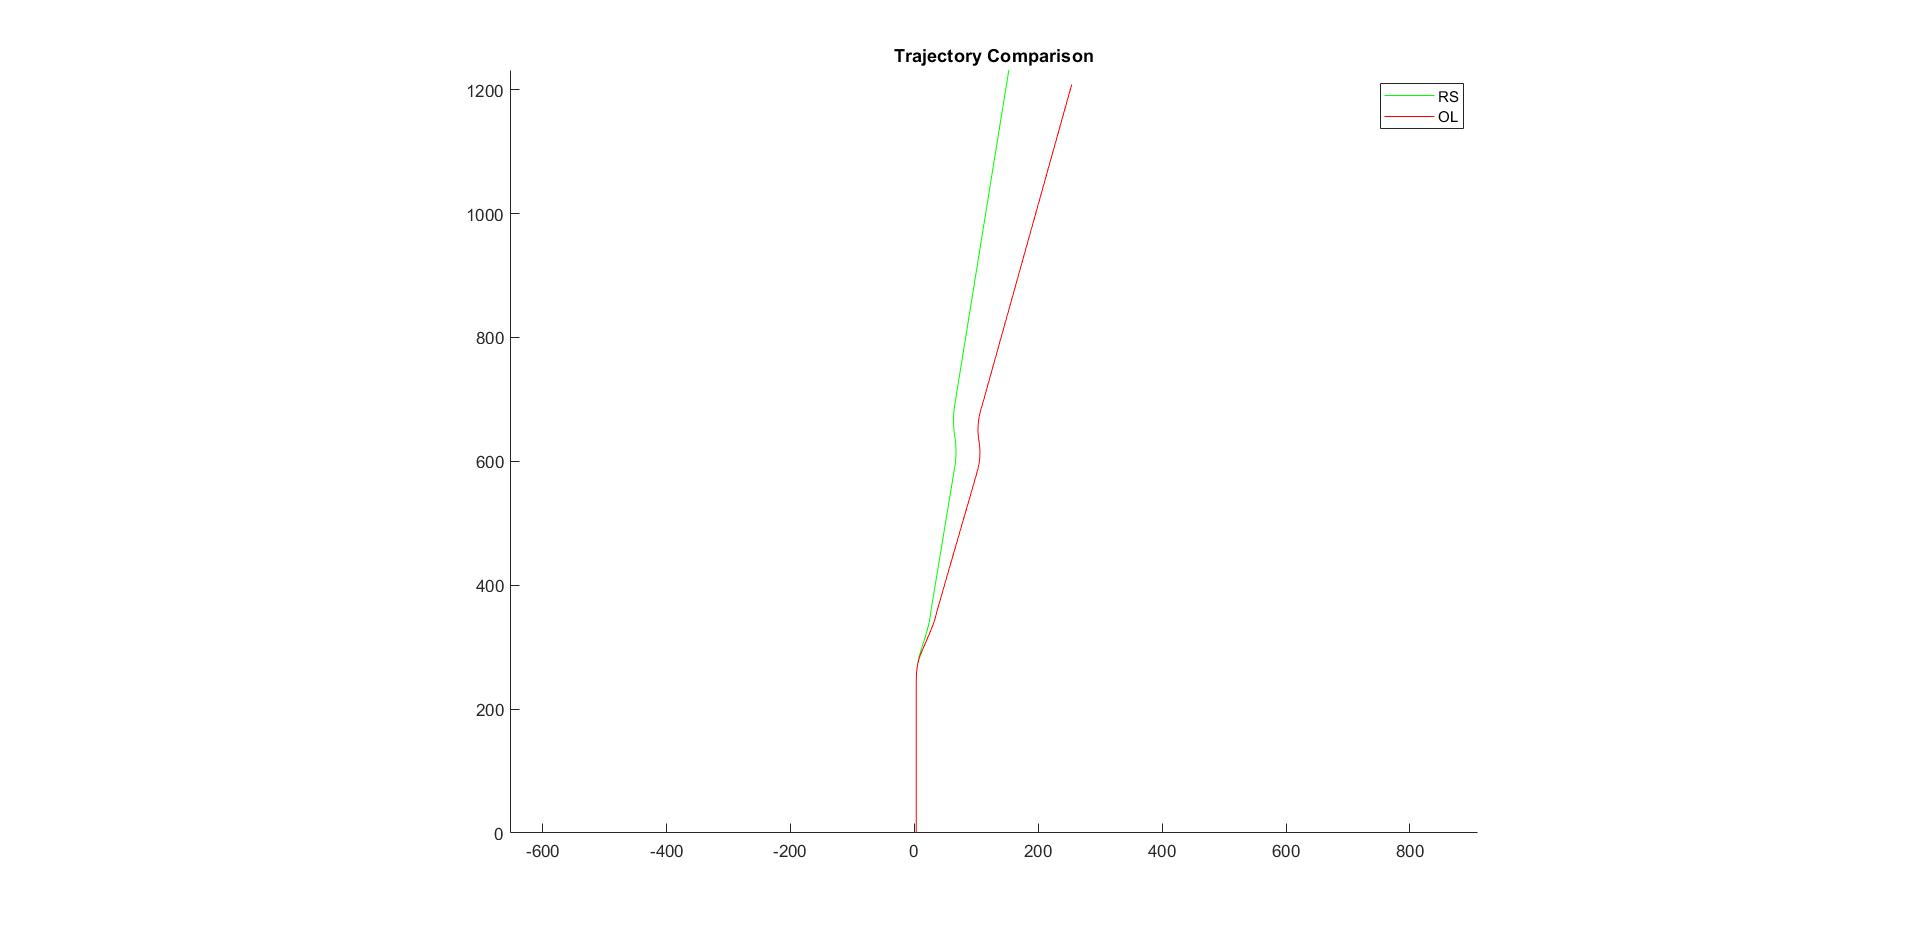
\includegraphics[scale=0.3]{./Images/LaneChangeIce/t} 
                \caption{(a)  RS vs OL comparison}
             
	\end{figure}

\begin{figure}[!h]
		\centering
	        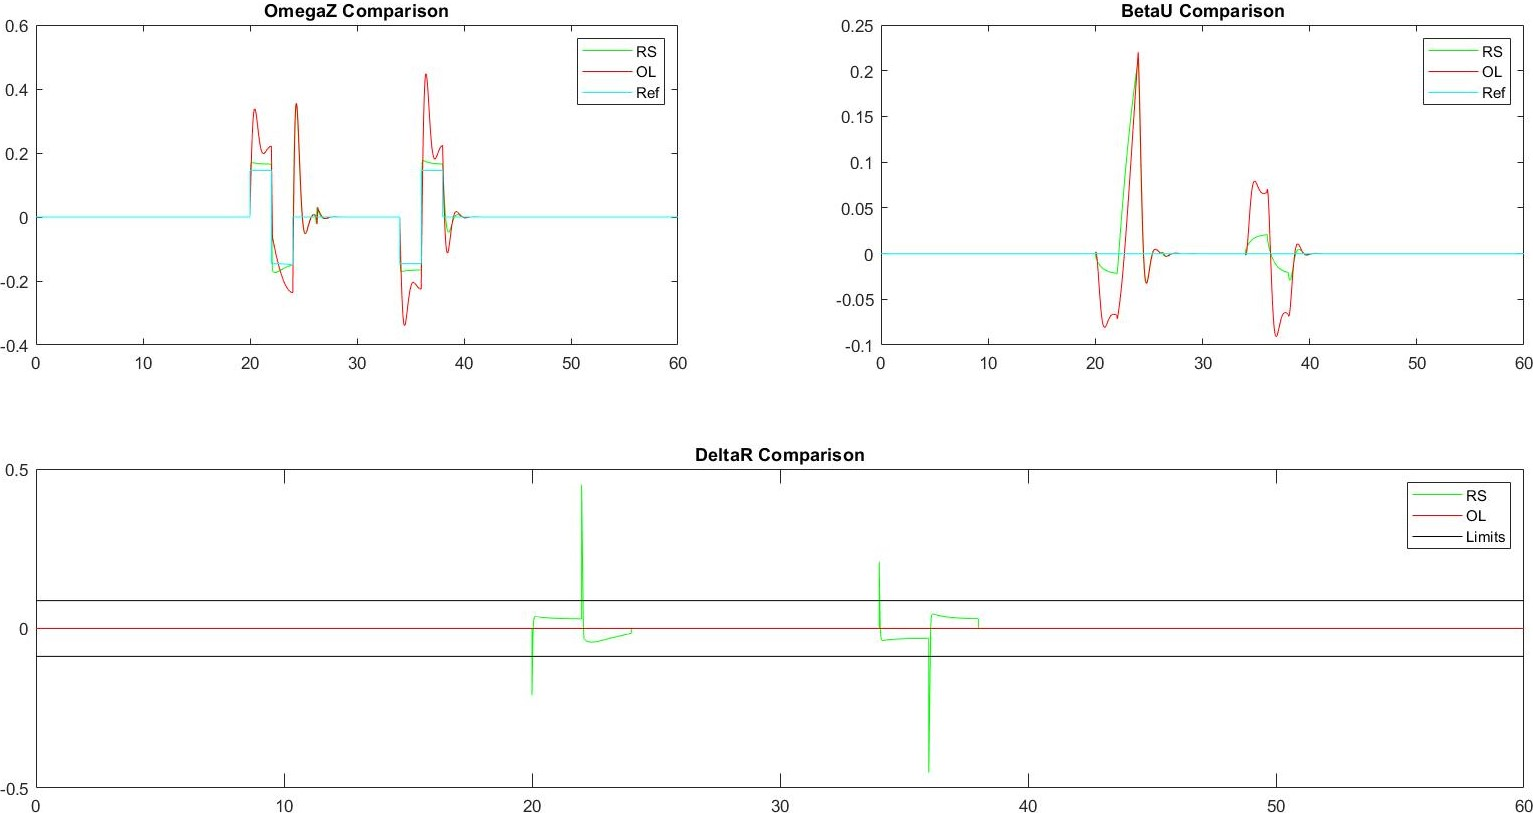
\includegraphics[scale=0.45]{./Images/LaneChangeIce/s} 
                \caption{(b) Comparison of $\beta_{u}$, $\omega_{z}$ and $\delta_{r}$} 
                \caption{Fig.5  Double turn in ice road}
        
 \end{figure}



    

\end{document}